\documentclass[12pt,a4paper,titlepage]{report}

\usepackage{times}

\usepackage[utf8]{inputenc}
\usepackage[T1]{fontenc}
\usepackage[romanian]{babel}

\usepackage{setspace}
\onehalfspacing

\usepackage[hidelinks]{hyperref}

\usepackage{graphicx}

\usepackage{minted}
%TODO: remove red box on parser error

\setminted{baselinestretch=1,fontsize=\footnotesize}

\usepackage{caption}

\usepackage{algorithm} %[plain] ?
\usepackage{algpseudocode}
\makeatletter
\renewcommand*{\ALG@name}{Pseudocod}
\makeatother

\usepackage{multirow}

\author{Barbu Paul - Gheorghe}

%TODO: coperta
%TODO: plan tematic?

\begin{document}

\begin{titlepage}
{
\centering
UNIVERSITATEA "LUCIAN BLAGA" DIN SIBIU\\
FACULTATEA DE INGINERIE \\
DEPARTAMENTUL DE CALCULATOARE ŞI INGINERIE ELECTRICĂ\\
}

\vfill

{
\centering
\Large
Secured Bootloader: program pentru controlul secvenței de
inițializare și al actualizării aplicației în microcontrollere
programabile
}

\vfill
{
\raggedright
Conducător ştiinţific: Conf. dr. ing. Morariu Daniel \\
%TODO: razvan?
Îndrumător: Conf. dr. ing. Morariu Daniel
}
\vfill

{
\raggedright
\hspace*{160pt}Absolvent: \\
\hspace*{160pt}Barbu Paul - Gheorghe\\
\hspace*{160pt}Specializarea:\\
\hspace*{160pt}Calculatoare și Tehnologia Informației
}

\end{titlepage}

\tableofcontents
\newpage

\subsection*{Prezentarea temei}

Lucrarea de față își propune dezvoltarea unui bootloader securizat pentru dispozitive embedded, aceste dispozitive conțin un microcontroller și în general utilizatorul respectivelor dispozitive nu vede și nu interacționează direct cu microcontroller-ul. Exemple de dispozitive embedded sau de aparate care conțin asemenea dispozitive: frigider, mașină de spălat, autoturism, termostat, contor electric, sistem de alarmă, sistem de supraveghere, ceasuri, etc.

Un bootloader este o aplicație care este în general încărcată pe microcontroller de către firma care vinde microcontroller-ul și care nu poate fi înlocuită ușor de către utilizatorii acestuia.
Rolul acestei aplicații este de a fi gazda ("host"-ul) și de a face verificările necesare încărcării unei alte aplicații pe microcontroller. În urma verificărilor se poate afirma că aplicația "guest" sau utilizator este una validă și că poate fi rulată de microcontroller cu încredere.
În urma procesului de bootloading ambele aplicații, atât bootloader-ul cât și aplicația utilizator, vor coexista în
memoria non-volatilă a dispozitivului embedded\footnote{în general pe flash-ul microcontroller-ului, conform unui memory map predefinit de producător}.
 
Motivele pentru care bootloader-ul este securizat și pentru care înlocuirea lui sau a aplicației utilizator
nu ar trebui să poată fi făcută de oricine țin în mică parte de protejarea proprietății intelectuale a celor ce creează aplicații guest pentru respectivul dispozitiv și într-o mai mare măsură țin de asigurarea integrității și a evitării modificării neautorizate a acestei aplicații pentru a asigura utilizatorului experiența pe care producătorul dispozitivelor embedded și-a imaginat-o. Acest lucru este crucial în ziua de astăzi, când criminalitatea în mediul cibernetic este în creștere\cite{interpol}\cite{morgan2016}. Consumatorii trebuie să poată fi protejați proactiv de acțiunile ilegale ale crackerilor, în antiteză cu metoda tradițională, reactivă care constă în schimbarea și îmbunătățirea unui sistem după ce acesta a fost compromis. Cele două metode se complementează reciproc, dar metoda proactivă are avantajul prevenirii unei acțiuni malițioase asupra sistemului informatic.

În afară de îmbunătățirea securității unui sistem embedded precum a fost descris mai sus, rolul bootloader-ului ar trebui să fie și de a mări flexibilitatea unui astfel de sistem. Acest rol este îndeplinit prin faptul că aplicația utilizator de pe microcontroller poate fi schimbată fără modificări hardware asupra sistemului. Schimbarea aplicației utilizator poate surveni din diverse motive, printre care: dezvoltatorul sistemului embedded hotărăște că este timpul să introducă funcționalități noi în aplicație sau că aplicația veche are unele defecte (bug-uri) care trebuie reparate sau chiar că sistemul embedded care înainte îndeplinea un rol trebuie să îndeplinească un rol complet nou, diferit față de cel vechi. Toate aceste scenarii implică folosirea bootloader-ului pre-instalat pe un dispozitiv pentru a încărca o altă aplicație (fie că e una complet nouă sau doar puțin modificată datorită remedierii defectelor din versiunea anterioară).

Bootloader-ul dezvoltat ar trebui să ne permită de asemenea reducerea costurilor. Prin costuri putem să considerăm de exemplu costurile survenite în urma livrării unui sistem embedded. Prin definiție mecanismele interne ale unui astfel de sistem nu sunt accesibile consumatorilor, deci orice modificare, fie ea chiar și software trebuie să fie făcută de producător. Așadar dispozitivul trebuie să fie livrat la producător, acesta aplică modificările și livrează înapoi dispozitivul clientului. Prin intermediul bootloader-ului ne propunem să putem face aceste modificări software la distanță. În esență aceste modificări se vor putea face independent, de către fiecare utilizator al sistemului.

Succint cerințele pe care trebuie să le satisfacă bootloader-ul sunt:
\begin{itemize}
\item asigurarea flexibilității dispozitivului embedded prin faptul ca aplicațiile de utilizator se pot schimba la nevoie
\item asigurarea securității și integrității unui sistem embedded în momentul în care aplicația este încărcată\footnote{securitatea sistemului depinde 100\% de aplicație în momentul în care aceasta rulează}
\item minimizarea costurilor de întreținere a dispozitivelor embedded dintr-un mediu industrial prin posibilitatea de a acționa bootloader-ul din exteriorul sistemului embedded
\end{itemize}

Prin rezolvarea acestor puncte, bootloader-ul va fi de ajuns de generic pentru aplicabilitate în diverse domenii și pe diverse platforme hardware. Fiind vorba de mediul embedded, bootloader-ul a fost proiectat și dezvoltat cu constrângerile de mărime în minte, cu atât mai mult cu cât pe un microcontroller se vor stoca două aplicații simultan, bootloader-ul și aplicația utilizator, dar doar una va rula la un moment dat.

\newpage
\chapter{Considerații teoretice}
\section{Introducere și etimologie}
Un bootloader se află pe orice sistem de calcul care trebuie să încarce un sistem de operare sau o aplicație terță.
Acest lucru este valabil fie că utilizatorul interacționează cu sistemul în timpul procesului de "boot" fie că procesul se petrece automat, fără interacțiune umană.

Cuvântul bootloader vine de la procesul de "boot" (sau "boot up"), care la rândul său este o scriere prescurtată a "bootstrap". Bootstrap în engleză semnifică "to pull oneself up by one's bootstraps", procesul prin care noi pornim la drum încălțându-ne. \cite{wikiBootstrap}

\section{Modul de funcționare al unui bootloader}
Orice bootloader trebuie stocat într-o memorie non-volatilă și de preferat disponibilă doar pentru citire, o memorie ROM\footnote{Read-Only Memory}, deoarece acesta trebuie să fie disponibil în momentul în care sistemul pornește indiferent de ce s-a întâmplat anterior pe sistem. Acest lucru garantează funcționarea corectă a sistemului și faptul că sistemul de operare sau aplicația utilizator poate fi schimbată. În caz contrar, când sistemul încetează să funcționeze din cauza unui defect (în general software) putem spune ca este "brick-uit", de la englezescul "brick" (cărămidă)\cite{wikiBrick}.

Un bootloader este, fără excepție, primul program executat de către un procesor, bine-înțeles cu excepția BIOS-ului\footnote{Basic Input/Output System} pe x86, dar putem ignora această particularitate, deoarece pe sistemele embedded, noțiunea de BIOS nu există.
În linii mari codul bootloader-ului este încărcat de pe discul solid\footnote{ROM la dispozitive embedded} în RAM\footnote{Random - Access Memory}, apoi este executat, iar în urma execuției acestui cod (în mod tipic un sector) se poate întâmpla unul din două lucruri:
\begin{enumerate}
\item bootloader-ul și-a încheiat treaba și a predat controlul aplicației utilizator respectiv sistemului de operare
\item bootloader-ul nu încape într-un sector și codul executat anterior este doar auxiliar
\end{enumerate}
Prima variantă este cea trivială. În al doilea caz avem de a face cu un așa zis "two stage bootloader", în primul stagiu făcându-se doar apelul spre acest stagiu secundar. Aici se va face de fapt încărcarea aplicației utilizator. Motivul din spatele încărcării în două faze este faptul că, fără drivere de disc și fără sisteme de fișiere, unitatea maximă pe care procesorul o poate citi de pe hard disc este sectorul, așadar intervin limitări legate de mărimea codului care poate fi executat la un moment dat.

Posibila diferență la sistemele embedded este aceea că microcontroller-ul poate executa cod direct din memoria flash și că bootloader-ul este probabil mai mic ca un sector, deoarece aplicațiile sunt reduse ca dimensiune și ca periferice cu care pot interacționa, display-ul și tastatura nefiind necesare în astfel de sisteme în timpul procesului de boot up.

La calculatoarele personale un bootloader bine cunoscut și pentru care avem nevoie de display și tastatură este GNU GRUB, folosit de majoritatea distribuțiilor GNU/Linux. Acest bootloader este vizibil utilizatorului (pe ecran, prin intermediul unui meniu asemănător cu cel din figura \ref{grub2menu}), iar în cazul sistemelor dual-boot sau multi-boot se poate chiar schimba sistemul de operare ce urmează a fi încărcat, acest lucru se face folosind tastatura.
\begin{figure}[h]
    \centering
    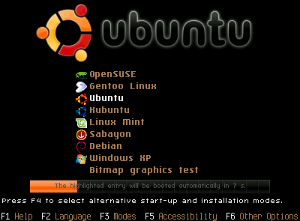
\includegraphics{grub}
    \caption{Meniul GRUB2}
    \label{grub2menu}
\end{figure}

\section{Studiu de caz: secvența de boot la PC}
Deși nu este în domeniul bootloader-ului, datorită omniprezenței acestor tipuri de procesoare merită să ne familiarizăm cu secvența de pași pe care un procesor din familia x86 o execută atunci când este pornit.
Această secvență fiind în strânsă relație cu pornirea bootloader-ului.

La pornire procesorul intră în modul real și execută instrucțiunea de la adresa \texttt{0xFFFFFFF0}\footnote{pe sisteme 32 si 64 bit} \cite{intel80386} \cite{intel64}. În mod normal această locație conține o instrucțiune de salt la locația de start a BIOS-ului care se află într-o memorie ROM.
BIOS-ul este de fapt primul program care se execută pe această arhitectură, nu direct bootloader-ul, în contradicție cu ceea ce am precizat anterior. Rolul BIOS-ului este de a inițializa hardware-ul și de a-l abstractiza, acesta rămânând tot timpul în funcțiune \cite{wikiBootSeq}.

Pasul de inițializare făcut de BIOS, poartă denumirea de POST\footnote{Power-On Self Test}, pas în care BIOS-ul pregătește memoria RAM și bus-urile pentru a putea începe comunicația cu perifericele a căror prezență urmează să o verifice. Aceste verificări sunt necesare, deoarece contrar unui sistem embedded, într-un calculator personal pot apărea și dispărea componente de la o pornire la alta, de exemplu putem adăuga o placă de rețea sau putem scoate placa video dedicată, în oricare dintre aceste cazuri BIOS-ul trebuie să știe de prezența unui periferic nou sau de lipsa unuia vechi pentru a putea prezenta toate aceste informații nivelelor superioare, care vor pune în funcțiune perifericele respective.
\begin{figure}[h]
    \centering
    \includegraphics{structuraPC}
    \caption{Structura "cochilie" a PC-ului}
    \label{shellArchitecture}
\end{figure}
Se poate observa în figura \ref{shellArchitecture} că BIOS-ul abstractizează hardware-ul, acest lucru este făcut mai departe și de sistemul de operare prin intermediul driverelor și prin intermediul apelurilor de sistem\footnote{"syscalls" sau "system calls" în engleză}. Datorită poziționării lor în centrul cochiliei, din aceeași figură reiese că aplicațiile beneficiază de cel mai mare nivel de abstractizare, ele nu trebuie să știe detalii intime despre așezarea datelor pe hard disk, în schimb au la dispoziție conceptul de fișier, indiferent de câte sectoare ocupă un asemenea fișier sau cum se comandă citirea lui la nivelele inferioare ale arhitecturii.

După inițializarea perifericelor, BIOS-ul trece printr-o listă pre-configurată de dispozitive de stocare non-volatile
până când găsește unul boot-abil. Un asemenea dispozitiv este caracterizat de faptul că ultimii doi octeți ai primului sector sunt egali cu \texttt{0x55AA}, aceasta reprezentând "semnătura" unui disc boot-abil.
Cel mai probabil această secvență \texttt{0x55AA} a fost aleasă deoarece în binar ea arată așa: \texttt{0101 0101 1010 1010}, observăm că biții sunt destul de variați, schimbarea în cascadă a lor neproducând din nou aceeași valoare și putând evita astfel încărcarea unui sector invalid sau corupt.

Odată ce discul boot-abil a fost găsit, primul lui sector este încărcat în memorie și executat, aici se află în sfârșit bootloader-ul. Codul este încărcat la adresa \texttt{0x0000:0x7C00} \cite{biosMBRaddr}.

În urma execuției bootloader-ul poate alege în mod automat de unde încarcă sistemul de operare sau, în cazul multi-boot, pasează această responsabilitate utilizatorului, punându-l să aleagă sistemul de operare dorit dintr-o listă.

În acest prim sector se află MBR-ul\footnote{Master Boot Record}. În cele mai multe cazuri cu o dimensiune de 512 octeți, MBR-ul conține de fapt codul bootloader-ului și detalii despre partiționarea discului\cite{norton99}. Codul bootloader-ului poate fi acela al lui GRUB sau bootloader-ul instalat de sistemele de operare Windows.

Structura MBR-ului este prezentată în tabelul \ref{mbrStruct}.

\begin{table}[h]
    \begin{tabular}{ | c | c | c | }
        \hline
        \textbf{Adresă} & \textbf{Descriere} & \textbf{Mărime (octeți)} \\ \hline
        \texttt{0x000} & Codul bootloader-ului & 446 \\ \hline
        \texttt{0x1BE} & Prima tabelă de partiție & 16 \\ \hline
        \texttt{0x1CE} & A doua tabelă de partiție & 16 \\ \hline        
        \texttt{0x1DE} & A treia tabelă de partiție & 16 \\ \hline
        \texttt{0x1EE} & A patra tabelă de partiție & 16 \\ \hline
        \texttt{0x1FE} & Primul octet al semnăturii discului (\texttt{0x55}) & 1 \\ \hline
        \texttt{0x1FF} & Al doilea octet al semnăturii discului (\texttt{0xAA}) & 1 \\ \hline
    \end{tabular}
    \centering
    \caption{Structura MBR-ului}
    \label{mbrStruct}
\end{table}

Din tabelul \ref{mbrStruct} se poate observa de asemenea că bootloader-ul este în realitate constrâns la mai puțin de 512 octeți, deoarece MBR-ul conține atât semnătura unui disc boot-abil, folosită de BIOS, cât și informații despre partițiile primare existente pe mediul de stocare. Pe scurt, tabelele de partiții au structura din tabelul \ref{partitionTableStruct} \cite{wikiPTE} și ele indică unde începe și unde se termină o partiție pe disc, cât și tipul acesteia și faptul că ea conține sau nu un sistem de operare, informație folosită apoi de bootloader pentru a popula lista de sisteme de operare disponibile pe calculator. Așadar dacă bootloader-ul, în urma inspectării tabelelor de partiții, găsește doar una activă, o va alege automat, în caz contrar îi va prezenta utilizatorului o listă cu sistemele de operare (respectiv partițiile pe care se află acestea) spre a face alegerea.

\begin{table}[h]
    \begin{tabular}{ | c | p{8cm} | c | }
        \hline
        \textbf{Adresă} & \textbf{Descriere} & \textbf{Mărime (octeți)} \\ \hline
        \texttt{0x0} & Partiție activă sau nu (conține sau nu un sistem de operare) & 1 \\ \hline
        \texttt{0x1} & Adresa Cilindru-Cap-Sector de început a partiției & 3 \\ \hline
        \texttt{0x4} & Tipul partiției & 1 \\ \hline
        \texttt{0x5} & Adresa Cilindru-Cap-Sector de final a partiției & 3 \\ \hline
        \texttt{0x8} & Adresa logică a blocului (LBA) de început a partiției & 4 \\ \hline
        \texttt{0xC} & Numărul de sectoare al partiției & 4 \\ \hline
    \end{tabular}
    \centering
    \caption{Structura sumară a unei tabele de partiție}
    \label{partitionTableStruct}
\end{table}

Observăm că toate aceste detalii teoretice cu privire la modul de funcționare al unui bootloader și al secvenței de inițializare la sistemele Intel x86 provin din limitarea intrinsecă a bootloader-ului la numai câteva sute de bytes de cod executabil. Pentru a ocoli această limitare s-a dezvoltat bootloader-ul în două stagii. Totuși în sistemele mai noi s-a dezvoltat standardul UEFI\footnote{Unified Extensible Firmware Interface: \url{http://www.uefi.org/}}. Acesta specifică 
un înlocuitor pentru BIOS și poate fi folosit pe o gamă mai largă de arhitecturi, inclusiv ARM, ARM64 și Itanium\cite{uefiSpec}. Este la latitudinea companiilor care comercializează sisteme de calcul să implementeze acest standard, care nu mai are limitările specifice BIOS-ului, acesta putând lucra direct cu fișiere și asigură extensibilitatea procesului de boot,  nu prin încărcarea succesivă a codului în două etape, ci prin aplicații care apelează și respectă interfața standard UEFI, similar unui sistem de plugin-uri.
Spre exemplu UEFI permite pornirea unui terminal de depanare, în cazul în care sistemul nu bootează se pot face investigații direct de la nivelul firmware-ului. De asemenea UEFI permite așa numitul "secure boot" \cite{uefiSpec} care permite încărcarea doar sistemelor de operare cu o semnătură digitală validă, acesta fiind un mecanism de protecție împotriva rulării unui sistem de operare modificat în scopuri malițioase, dar poate fi folosit și ca mecanism de împiedicare a instalării altor sisteme de operare care nu sunt vândute de un anumit producător deoarece acele sisteme de operare nu vor fi validate de mecanismul securizat de boot al UEFI \cite{zdnetSecureBoot}.

\subsection{Variante de bootloader}

În afară de bootloader-ul instalat de sistemele de operare Windows, numit Windows Boot Manager, și de GNU Grub, ambele prezentate anterior, mai există și alte variante de bootloader-e care pot fi instalate pe un sistem de calcul.

Toate aceste bootloader-e diferă în mărime și in funcționalitate, dar în final, toate au același scop: de a găsi și de a porni un sistem de operare.

Sistemul de operare poate fi localizat pe rețea, de exemplu Grub și Syslinux au capabilitatea de a încărca sistemul de operare dintr-o locație centralizată, lucru util în cazul în care un administrator de sistem dorește controlul asupra mai multor sisteme, fără să le administreze manual pe fiecare în parte.

De asemenea anumite bootloader-e pot încărca aplicații sau sisteme de operare comprimate, stocate așa deoarece este posibil ca spațiul să fie limitat, cum este cazul sistemelor embedded. Pentru aceste sisteme a fost dezvoltat bootloader-ul "Das U-Boot" \footnote{http://www.denx.de/wiki/U-Boot/} care poate fi folosit pe o multitudine de arhitecturi și care se axează pe minimizarea mărimii codului și a timpilor de rulare prin simplitatea codului\footnote{http://www.denx.de/wiki/U-Boot/DesignPrinciples}. Urmărirea acestor principii de dezvoltare au făcut ca acest bootloader să fie prezent într-o gama largă  de produse, de la dispozitive industriale, până la echipamente de rețea, cum ar fi cele de la Ubiquiti Networks cât și la laptop-urile dezvoltate de Google, Chromebooks \cite{wikiUboot}.

\section{Studiu de caz: secvența de inițializare la un sistem embedded}

În ceea ce privește sistemele embedded, acestea fiind mai puțin performante față de un calculator personal, putem spune că și secvența de inițializare a lor și respectiv bootloader-ul sunt mai puțin complexe.
Acest lucru este datorat și tipurilor de periferice și dispozitive de stocare cu care sistemul este dotat. În cazul dispozitivelor embedded perifericele ca tastatura sau mouse-ul și monitorul, nu există, iar mediile de stocare sunt in general memorii flash, nu hard disk-uri, făcând accesul la date mult mai simplu și nefiind nevoie de nivelele de abstractizare pe care le oferă BIOS-ul și sistemul de operare.

În general când lucrăm cu un microcontroller, nu există conceptul de bootloader, ci doar conceptul de inițializare al hardware-ului, lucru care este deja implementat de către bibliotecile oferite de producător.
Așadar, când un microcontroller este resetat acesta execută câțiva pași bine definiți pentru a executa codul încărcat (flash-uit) de către dezvoltator, procesul este similar cu cel prezentat anterior pentru arhitecturile x86, dar în mare parte este mai simplu. Simplitatea se trage din faptul ca acest cod de inițializare nu trebuie să verifice în mod dinamic existența unor noi periferice sau lipsa unora vechi deoarece sistemul embedded nu este deschis extensibilității pentru utilizator, acesta este mult mai rigid.

Pentru acest studiu de caz vom considera core-ul M7 de la ARM\footnote{https://www.arm.com/products/processors/cortex-m/cortex-m7-processor.php} împreună cu secvența de inițializare aferentă lui.
Ca pentru orice procesor și pentru acest model există o tabela a vectorilor de întrerupere\footnote{IVT - Interrupt Vector Table}, care nu este altceva decât o zonă de memorie care conține la anumite adrese pointeri spre rutinele de tratare a întreruperilor. În cazul core-ului M7 primele două locații din această tabelă sunt valorile inițiale ale registrului Stack Pointer\footnote{abreviat SP} și ale registrului Program Counter\footnote{abreviat PC sau IP (Instruction Pointer)} \cite{kv5x}.
Combinația celor două registre ne permite să putem începe execuția codului, deoarece Program Counter-ul ne indică adresa următoarei instrucțiuni care trebuie executată de către procesor. Stack Pointer-ul ne indică locația în memorie unde se află vârful stivei, zona de memorie folosită pentru a stoca parametrii unei funcții și date despre locația unde trebuie să revenim din funcția apelată.

În listing-ul \ref{ivt-m7} putem vedea, în cod asamblare, modul în care rutinele de tratare a întreruperilor sunt declarate.
\begin{listing}[h]
\begin{minted}{asm}
__isr_vector:
  .long __StackTop
  .long Reset_Handler
  .long NMI_Handler
  .long HardFault_Handler
  .long MemManage_Handler
  .long BusFault_Handler
  .long UsageFault_Handler
\end{minted}

\caption{Începutul tabelei vectorilor de întrerupere}
\label{ivt-m7}
\end{listing}

Prima intrare din acest vector este valoarea inițială a stack pointer-ului, numit aici \texttt{\_\_StackTop}, acesta nu este un pointer spre o rutină de tratare a unei intreruperi, ci are doar rolul de a indica unde începe zona de memorie rezervată stivei. În schimb cea de a doua intrare în interrupt vector table este într-adevăr un pointer spre o astfel de procedură.
Aceasta este apelată de fiecare dată când procesorul primește semnalul de reset. Din acest motiv putem spune ca PC-ul inițial se află pe poziția a doua în tabelă, deoarece el corespunde acestei rutine.

Continuând pe firul execuției în urma resetării microcontroller-ului, rutina \texttt{Reset\_Handler} nu face altceva decât să 
apeleze funcția \texttt{SystemInit} care este responsabilă cu inițializarea cache-urilor și a unității de procesare a numerelor cu virgulă flotantă. În urma acestui apel controlul este redat rutinei \texttt{Reset\_Handler} care mai departe se va ocupa cu copierea secțiunii de constante a codului în memoria RAM și de inițializarea zonei de memorie rezervată pentru heap (folosită când programul alocă dinamic memoria). De asemenea \texttt{Reset\_Handler}-ul continuă cu apelul funcției \texttt{\_\_libc\_init\_array} (care inițializează structurile necesare limbajului C) și în final va apela punctul unic de intrare într-un program, funcția scrisă de dezvoltator: \texttt{main}.
Codul pentru pașii de inițializare se află în fișierul \texttt{startup\_MKV58F24.S} din directorul \texttt{startup} al unei aplicații embedded\footnote{Locația depinde de producătorul microcontroller-ului și de mediul de programare folosit}.

După ce se apelează \texttt{main}-ul, practic controlul îi este predat aplicației scrisă de dezvoltator și secvența de inițializare a luat sfârșit. În afară de memorie și de componentele auxiliare acesteia, cache-urile, alte componente ale microcontroller-ului nu au fost pornite, acest lucru se datorează faptului că responsabilitatea aceasta este predată aplicației . Lucru necesar pentru a consuma cât mai puțină energie posibil, dacă aplicația nu va folosi, spre exemplu, comunicația pe portul serial, nu va inițializa acest port, ceea ce va duce la evitarea consumului de energie fără scop.

\inputminted{asm}{reset_handler.s}
\captionof{listing}{Definiția rutinei Reset\_Handler\label{resetHandler}}

\begin{figure}[h]
    \centering
    \includegraphics[width=0.75\textwidth]{structuraEmbedded}
    \caption{Structura "cochilie" a unui sistem embedded}
    \label{shellEmbedded}
\end{figure}

Secvența descrisă anterior se poate vedea sub formă de schemă logică în figura \ref{shellEmbedded} și sub formă de cod asamblare în listingul \ref{resetHandler}.
Am păstrat în această figură și analogia structurii cochilie pentru a ilustra diferența majoră între un sistem embedded care funcționează pe o arhitectură ARM\footnote{în cazul de față Cortex M7} și arhitectura x86 folosită în calculatoarele personale și server-e. Diferența constă în faptul că în cazul programării dispozitivelor embedded sistemul nu include nivele de abstractizare pe care programatorul nu le cere și de care nu are nevoie în mod explicit. În mod implicit sistemele embedded nu oferă altceva decât biblioteci care ne dau acces la hardware, la registrele microprocesorului. Prin aceste registre se pot controla porturile de comunicație\footnote{UART, SPI, I2C}, se poate scrie sau șterge memoria flash, putem controla convertoarele analog-digitale și pe cele digital-analogice, etc. Bine-înțeles că există producători care oferă un nivel mai ridicat de abstractizare prin biblioteci, un asemenea producător este NXP\footnote{\url{http://nxp.com/}}. Aceste biblioteci ascund lucrul cu registrele microcontroller-ului în favoarea lucrului cu funcții și structuri\cite{ksdk}, ele reprezintă chiar echivalentul BIOS-ului și al colecției de driver-e în sistemele x86, deoarece scopul lor este similar: de a abstractiza hardware-ul pe care aplicația rulează.

Un programator embedded are la dispoziția sa și sisteme de operare, în principal de tipul "real time"\footnote{de timp real}.
Aceste sisteme de operare sunt caracterizate de predictibilitatea lor și de garanțiile puternice pe care le fac legat de timpul în care termină de executat un task\cite{silberschatz}.

Totuși modul în care acestea sunt folosite diferă substanțial față de modul în care sistemele de operare non-real-time sunt folosite. Acest lucru este datorat faptului că un sistem de operare real-time folosit pe o platformă embedded va fi o parte a aplicației scrisă de dezvoltator, nu există deja un mediu pre-definit în care aplicația este creată, ca la sistemele de operare de uz general. Asta înseamnă că sistemul de operare real-time va fi inclus în aplicație la nivelul codului sursă sau link-at static la aceasta, astfel că funcționalitățile lui sunt accesate asemenea funcționalităților unei biblioteci, prin apeluri de funcții și structuri de date, din nou revenind la analogia anterioară, unde bibliotecile țin loc de BIOS, drivere, și acum, chiar și de sistem de operare real-time \cite{freertos}. 

Acest mod de lucru nu este totuși unic industriei embedded, el poate fi observat într-o oarecare măsură și în cadrul așa numitului unikernel. Un unikernel reprezintă o aplicație de uz general \cite{barbu} și un nucleu de sistem de operare, combinate într-o singură unitate funcțională care poate servi drept firmware-ul unui dispozitiv. Față de cazul embedded, unde sistemul de operare era inclus în aplicație (fie la nivel de cod sursă, fie link-at static), aici lucrurile stau invers, aplicația va fi inclusă direct în sistemul de operare de uz general prin linkare statică. Acest lucru duce la efectul secundar de a putea integra o singură aplicație în unikernel, de unde provine și numele, un nucleu de sistem de operare dedicat unei singure aplicații \cite{kantee}.

%TODO: reitereaza ideea asta la capitolul cu practica
După cum am văzut în listingul \ref{resetHandler}, funcția main este chemată direct, fără să se facă o selecție dintr-o colecție de funcții (corespondente unor aplicații) disponibile, similar cu selecția sistemului de operare de către bootloader.
Putem modifica acest lucru prin introducerea unui strat de abstractizare suplimentar. Adică să scriem o aplicație care să fie apelată implicit de către microcontroller, iar apoi această aplicație să joace rolul de bootloader. Bootloader care va fi responsabil cu alegerea unei aplicații pe care să o ruleze și eventual cu validarea acesteia similar cu sistemul UEFI.

În urma alegerii și validării aplicației, bootloader-ul va trebui să îi predea controlul acesteia, similar unui bootloader pentru arhitecturile x86 care predă controlul sistemului de operare. Totuși fiind vorba de dispozitive embedded rareori este necesar ca bootloader-ul să aleagă între două aplicații guest pe care să le ruleze, așa cum se întâmplă la calculatoarele personale cu bootloader-ul și sistemele de operare. Acest lucru este cauzat de hardware-ul redus ca putere și spațiu de stocare, dar și de o caracteristică intrinsecă a sistemelor embedded: orientarea spre un singur domeniu și rezolvarea unui singur fel de problemă la un moment dat. Așadar este mai probabil ca în bootloader-ele embedded să vedem modalități de a încărca o aplicație complet nouă pe microcontroller (care o înlocuiește pe cea veche) în locul funcționalității de a alege o aplicație dintr-o colecție pre-existentă.

În funcție de tipul microcontroller-ului aplicația se poate încărca folosind un tip de comunicație serială clasică, precum UART, I2C și SPI sau prin metode întâlnite mai des pe sistemele de uz general cum ar fi USB-ul și Ethernet-ul.

\subsection{Variante de bootloader}

Similar arhitecturilor generale, există de asemenea diverse bootloader-e create pentru dispozitive embedded. "Das U-Boot", precizat și în secțiunea anterioară este unul dintre ele, printre principiile acestuia de design aflându-se și portabilitatea.

Printre alte alternative se numără și "KBoot", bootloader-ul celor de la Kinetis. Spre deosebire de "Das U-Boot", acesta este creat special pentru dispozitivele dezvoltate de NXP \cite{kboot}. Procesul de inițializare este similar cu cel descris anterior. Microcontroller-ul pornește și începe să execute codul bootloader-ului, care la rândul său așteaptă să primească o aplicație pe care să o încarce pe toată gama de porturi disponibile pe dispozitiv. În urma încărcării aplicația este pornită. Ceea ce este special la acest bootloader este faptul că el poate fi folosit și drept sistem de control al dispozitivului, permițând rularea unor comenzi administrative cum ar fi citirea anumitor zone de memorie, ștergerea lor și scrierea de date. Bootloader-ul pune la dispoziție și o aplicație similară unui terminal prin care pot fi executate aceste comenzi.

Un alt bootloader embedded este \guillemotleft$\mu$Tasker "Bare-Minimum" Boot Loader\guillemotright, acesta după cum îi spune și numele conține doar minimul necesar pentru a încărca o altă aplicație \cite{uTaskerMinim}. El se bazează pe "$\mu$Tasker Serial Loader" pentru a face încărcarea prin Ethernet, UART sau chiar și de pe carduri de memorie \cite{uTaskerSerial}. Deoarece  încărcarea se face în doi pași, primul făcând minimul necesar și într-un spațiu cât mai mic, iar cel de-al doilea pas făcând încărcarea propriu zisă putem spune că acest bootloader se aseamănă cel mai mult cu bootloader-ele pentru arhitecturi x86, precum GRUB.

\section{Protecția și securitatea}
Unul dintre scopurile pe care bootloader-ul dezvoltat în cadrul acestei lucrări și le propune să le atingă este acela de a asigura integritatea și de a evita modificarea neautorizată a aplicației pe care bootloader-ul o va încărca.

Deducem deci două categorii de modificări care pot surveni asupra aplicației:
\begin{enumerate}
\item modificarea ne-intenționată datorată problemelor de transmisie spre microcontroller;
\item modificarea intenționată, posibil pentru a rula cod malițios.
\end{enumerate}

Vom studia în cele ce urmează posibile soluții pentru aceste două probleme.

\subsection{Coduri polinomiale}
Pentru a preveni prima categorie de modificări, cele datorate mediului de comunicație, soluțiile trebuie să acționeze la nivelul pachetelor care se transferă între microcontroller și calculator (dacă presupunem de exemplu o transmisiune serială, RS232). În timpul transferului de date, datorită interferențelor, anumiți biți pot ajunge schimbați la destinație. Pentru a detecta astfel de erori avem la dispoziție mai multe tehnici.

Cea mai simplă tehnică ar fi introducerea unui bit de paritate de către expeditor, bit pe care destinatarul trebuie să îl verifice pentru a avea siguranța că datele au fost transmise corect. Această tehnică poate detecta schimbarea unui singur bit. Este deci o metodă simplă, nu adaugă meta-date, în afară de bit-ul de paritate, datelor utile. Un exemplu ar fi dacă dorim să transmitem șirul de biți \texttt{0101 1010} cu paritate pară, atunci acesta ar deveni: \texttt{0101 1010 0}, iar cu paritate impară ar deveni: \texttt{0101 1010 1}. Observăm că în primul caz, cel al parității pare, numărul total de biți setați (cu valoarea 1) este par și am adăugat la final un bit de 0, iar în cazul parității impare, numărul transmis de biți cu valoarea 1 este impar deoarece am adăugat la final un bit de 1. Totuși acestă metodă nu este de ajuns pentru a detecta dacă mai mulți biți au fost afectați de erori, după cum se poate vedea în cazul următor: dacă dorim să transmitem secvența de biți \texttt{0101 1010} cu paritate pară vom transmite secvența \texttt{0101 1010 0}. În timpul transmisiei, datorită interferențelor doi biți se modifică din 1 în 0: \texttt{0000 1010 0}, făcând astfel datele care ajung la destinatar să fie diferite față de cele expediate, dar cu un bit de paritate încă valid și drept consecință făcând imposibilă detectarea erorilor.

În urma acestor limitări W. Wesley Peterson a descoperit un algoritm mai complex de detecție a erorilor, numit cyclic redundancy check\footnote{CRC}, "coduri ciclice" sau "coduri polinomiale" \cite{wikiCrc}. Rezultatul acestui algoritm este, similar cu bit-ul de paritate, adăugat datelor utile (de unde vine și denumirea de "redundant", deoarece nu adaugă date noi, ci reprezintă o transformare a celor existente deja). Codurile ciclice sunt mai versatile deoarece acestea pot detecta erori în secvențe mai lungi de un bit. Acest algoritm de detecție al erorilor este folosit și la nivelul "Data Link"\footnote{legătură de date} al modelului ISO-OSI datorită capacității lui bune de a detecta erori.

Rezultatul unui CRC este reprezentat pe un număr fix de biți, de exemplu unele dintre cele mai folosite astfel de coduri polinomiale sunt CRC-8, CRC-16 și CRC-32, cu reprezentări pe 8, 16 și respectiv 32 de biți. Lungimea acestora este aleasă în funcție de cât de bună dorim să fie detecția și de cât de multe meta-date dorim să adăugăm mesajului util. De regulă codul polinomial poate detecta erori de o lungime maximă cu lungimea proprie de reprezentare, de exemplu CRC-32 poate detecta maxim un șir de 32 de biți alăturați care au fost modificați în timpul transferului.

CRC-urile se mai numesc coduri polinomiale deoarece polinoamele sunt fundamentul matematic pe care se bazează. Algoritmul care calculează CRC-ul tratează un șir de biți ca fiind coeficienții unui polinom de ordin n+1.
Așadar șirul de biți \texttt{0000 00111} corespunde polinomului $x^8 + x^2 + x + 1$, prin convenție cel mai semnificativ bit este tot timpul 1 fără să fie reprezentat (aici coeficientul lui $x^8$), de aceea de exemplu algoritmul CRC-8, cu rezultatul reprezentat pe 8 biți are de fapt 9 membrii în polinom. Operațiile aritmetice cu polinoame se fac în "modulo 2", ceea ce înseamnă că nu există carry pentru adunare și împrumuturi pentru scădere. Acest lucru face ca adunarea și scăderea să fie echivalente cu operația de sau-exclusiv \cite{tanenbaumCN}. Pentru a calcula CRC-ul unui șir de biți, atât destinatarul cât și expeditorul trebuie să stabilească un polinom comun pe care să îl folosească la generarea CRC-ului, acest polinom se numește sugestiv: polinom generator. Polinomul generator este folosit ca împărțitor, iar biții datelor utile sunt folosiți pentru a construi polinomul deîmpărțit. În urma operației de împărțire între cei doi termeni, doar restul se va folosi, el este CRC-ul și este reprezentat pe n biți, unde n+1 este ordinul polinomului generator. Este important să subliniem că împărțirea polinoamelor are loc în aritmetică modulo 2, acest lucru făcând facilă implementarea algoritmului de calcul al unui CRC în hardware, acesta necesitând doar registre de shiftare și porți XOR \cite{hackersDelight}.

Din punct de vedere software o funcție în limbajul C care calculează un CRC pe 16 biți este prezentată în listing-ul \ref{crcInC}. Din cod se poate vedea cum pentru fiecare bit, al fiecărui octet din datele de intrare, celui mai semnificant bit al CRC-ului și bit-ului de date le sunt aplicate operația de sau-exclusiv și apoi CRC-ul este shiftat la stânga cu o poziție \cite{rossCrc}.

\begin{listing}[h]
\begin{minted}{c}
uint16_t Crc16(const uint8_t *pu8Data, const uint32_t u32DataLen,
               const uint16_t u16Poly, uint16_t u16Crc)
{
    for(uint32_t byte=0; byte<u32DataLen; ++byte)
    {
        u16Crc ^= (*pu8Data++) << 8;
        for(uint8_t bit=0; bit<8; ++bit)
        {
            u16Crc = (u16Crc << 1) ^ ((u16Crc & 0x8000) ?
                                      u16Poly : 0);
        }
    }

    return u16Crc;
}
\end{minted}

\caption{Implementarea unei rutine de calcul a CRC-16}
\label{crcInC}
\end{listing}

Folosind algoritmul exemplificat în listing-ul \ref{crcInC} atât expeditorul cât și destinatarul vor calcula codul ciclic. Dacă destinatarul observă că valoarea CRC-ului diferă înseamnă că au apărut erori la trimiterea datelor și cere o re-transmisiune până când erorile nu mai apar. Datorită faptului că discutăm despre un sistem embedded codurile de corecție a erorilor nu au fost considerate spre implementare, ci doar cele de detecție a erorilor, prezentate anterior.

\subsection{Criptarea și autentificarea datelor}

Unul dintre scopurile bootloader-ului este reducerea costurilor prin acționarea sa "de la distanță". Pentru a face acest lucru dezvoltatorul de aplicații trebuie să îi trimită clientului o aplicație care să fie folosită de bootloader. Bine-înțeles acest lucru se poate face pe internet (de exemplu prin email sau upload pe web), dar expunerea aplicației pe web presupune riscul de a expune aplicația la modificări malițioase. O persoană cu rele intenții poate pune la cale un atac de tip man-in-the-middle\footnote{tradus literalmente: om în mijloc} în care clientul este practic păcălit că descarcă aplicația dezvoltatorului, dar de fapt descarcă un virus, care va fi apoi încărcat pe dispozitivul său. Datorită naturii sale embedded dispozitivul ar putea părea că își face treaba pe care a fost proiectat să o facă, dar, în plus, poate să adune și date despre utilizator sau chiar să permită controlul neautorizat asupra dispozitivului. Gradul de gravitate al acestei breșe de securitate diferă în funcție de dispozitiv și de întrebuințarea lui, dar ne dorim totuși să prevenim aceste modificări nedorite ale aplicației.

Trebuie să observăm că de data aceasta modificările aduse aplicației nu mai sunt ne-intenționate, ci intenționate, așadar nu mai putem sa folosim CRC-urile, având nevoie de un sistem dedicat pentru această gamă de probleme. Codurile polinomiale nu sunt o opțiune deoarece, în general, acestea se atașează la finalul datelor utile și pot fi recalculate cu ușurință, un atacator putând să schimbe o porțiune de cod și apoi să recalculeze CRC-ul și să îl înlocuiască pe cel original.

Soluția pe care o căutăm este una de natură criptografică. Pentru a evita orice fel de contact cu mediul exterior aplicația trebuie să fie criptată în momentul în care dezvoltatorul o publică și trebuie să fie decriptată doar pe dispozitivul embedded, de către bootloader. În acest mod dezvoltatorul și clientul pot fi siguri că aplicația nu poate fi modificată deoarece conținutul ei decriptat nu este expus niciodată. Standardul de criptare ales este Advanced Encryption Standard - Galois Counter Mode\footnote{AES-GCM} \cite{wikiAes} cu o cheie de 128 de biți deoarece acest standard se găsește implementat în biblioteci special create pentru mediul embedded\footnote{\url{https://tls.mbed.org/}} și, dacă este implementat corect, până acum nu s-a descoperit nicio vulnerabilitate practică asupra lui, metodele curente având o complexitate de timp de aproximativ $2^{120}$ \cite{bogdanov}.

Pe scurt, acest standard de criptare este bazat pe algoritmul Rijndael, dezvoltat de Joan Daemen și Vincent Rijmen \cite{rijndael}, modul de funcționare al algoritmului este prezentat în pseudocodul \ref{impl-aes}.

\begin{algorithm}
\begin{algorithmic}
\State n $\gets$ numărul de runde
\State keys $\gets$ generează cheile specifice fiecărei runde
\State S $\gets$ creează matricea de stare
\State \Comment{Runda inițială}
\State S $\gets$ S $\oplus$ keys[0]

\State \Comment{Rundele intermediare}
\State i $\gets$ 1
\While{i < n}
\State SubBytes(S)
\State ShiftRows(S)
\State MixColumns(S)
\State S $\gets$ S $\oplus$ keys[i]
\State i $\gets$ i + 1
\EndWhile
\State \Comment{Runda finală}
\State SubBytes(S)
\State ShiftRows(S)
\State S $\gets$ S $\oplus$ keys[n]

\end{algorithmic}

\caption{Pseudocodul algoritmului AES (Rijndael)}
\label{impl-aes}
\end{algorithm}

Pentru simplitatea explicației vom considera cazul particular AES-128. Algoritmul are nevoie de 10 iterații pentru a produce o criptare sigură a datelor de intrare, trebuie așadar să genereze 10 chei distincte pornind de la cheia de criptare inițială. Acest lucru se face folosind algoritmul "Rijndael key schedule", care împarte cheia de criptare în blocuri de 16 octeți, aranjați sub forma unei matrici. Pentru fiecare cheie, care corespunde unei alte runde, elementele matricii și anumite coloane sunt interschimbate, apoi sunt combinate (prin sau-exclusiv) cu alte elemente ale cheii anterioare. Se generează astfel chei distincte și dependente de cheia de criptare inițială.
După generarea cheilor specifice fiecărei runde, urmează ca datele de intrare care vor fi criptate să fie organizate în blocuri de 16 octeți, sub forma unei matrici, rezultând matricea de stare \texttt{S}.

În runda inițială această matrice este combinată cu cheia de criptare, iar apoi încep rundele intermediare, unde elementele matricii sunt substituite cu alte elemente (asemeni unui cifru Caesar), acesta este pasul \texttt{SubBytes}. Urmează permutarea circulară a liniilor din matrice (pasul \texttt{ShiftRows}) și pasul de amestecare a biților de pe o coloană, \texttt{MixColumns}. Ultima parte constă în combinarea noii matrici de stare cu cheia de criptare aferentă rundei în care se află algoritmul. Algoritmul se încheie cu runda finală, repetând aceeași pași, cu excepția celui de \texttt{MixColumns}.

Rezultatul criptării este matricea de stare, care este transformată înapoi într-un șir de biți. Acest șir, criptat fiind, pentru a-i afla semnificația, tebuie decriptat folosind procesul invers celui descris anterior. Proprietățile algoritmului Rijndael își au fundamentul în grupurile Galois și calculul cu polinoame, asemănător codurilor ciclice. Așadar pot fi implementate simplu în software și chiar și în hardware, cu unii producători de procesoare ca Intel și AMD care au introdus instrucțiuni speciale pentru criptarea și decriptarea AES \cite{intel64}.

Criptarea de una singură nu este totuși suficientă pentru a asigura și autenticitatea datelor. Ea poate doar să asigure doar confidențialitatea, pentru a asigura și integritatea datelor trebuie să folosim un "mod de operare" al algoritmului AES. Dorim să facem acest lucru deoarece metoda de transmisie a aplicației poate introduce erori sau datele criptate pot fi înlocuite de un atacator. 

Modul de operare pentru AES ales aici este AES-GCM, Galois/Counter Mode. Alegerea a fost făcută datorită faptului că modul acesta de operare este recomandat de Institutul Național de Standarde și Tehnologie al Statelor Unite\footnote{NIST - National Institude of Standards and Technology} \cite{nistGCM} și că a fost proiectat în așa fel încât să fie rapid \cite{gcmSpec}. Pentru a putea folosi AES-GCM, în afară de datele pe care vrem să le criptăm și autentificăm avem nevoie de o cheie cu care să criptăm datele (cheia trebuie păstrată secretă) și de un vector de inițializare\footnote{IV - Initialization Vector} pentru algoritmul de autentificare. Algoritmul de autentificare va folosi acest vector pentru a crea o etichetă unică (numită tag) a combinației datelor de intrare și vectorului de inițializare. Trebuie notat că această metodă este diferită de CRC-uri deoarece ea se bazează pe cheia de criptare și pe faptul că un potențial atacator nu are acces la ea, deci atacatorul nu poate pur și simplu să re-cripteze datele și să genereze un nou tag dacă nu are cheia de criptare corectă. Modul general de criptare și de decriptare, cât și fluxul datelor pe care se bazează AES-GCM este ilustrat în figura \ref{howAesWorks}

\begin{figure}[h]
    \centering
    \includegraphics[width=0.75\textwidth]{aes-gcm}
    \caption{Fluxul datelor între dezvoltator și client prin prisma AES-GCM}
\label{howAesWorks}
\end{figure}

De fiecare dată când se criptează date, pentru ca algoritmul să își păstreze proprietățile, vectorul de inițializare trebuie să fie diferit. Acesta, împreună cu tag-ul și cu datele criptate rezultate în urma rulării AES-GCM trebuie trimise spre destinatar, acesta va folosi IV-ul pentru a inițializa algoritmul și pentru a verifica dacă obține același tag ca cel primit de la expeditor, dacă o face, atunci datele primite sunt cele trimise de expeditor și nu au fost interceptate și modificate între timp. Evident este de importanță maximă ca sistemul să protejeze cheile de criptare, vom explora cum se poate face acest lucru în secțiunea următoare.

\section{Procesul de flashing al unui microcontroller și protecția cheilor de criptare}
După cum am aflat în secțiunea anterioară cheile de criptare trebuie să fie păstrate un secret, ele fiind elementul de bază al securității, algoritmul de criptare devine irelevant dacă cheile nu sunt păstrate în siguranță.
Într-o instanță ele se află pe sistemele dezvoltatorului, pe care le considerăm sigure și private. Aceste sisteme sunt folosite pentru criptarea aplicației care va fi folosită de bootloader și care va rula la final pe microcontroller. Într-o altă instanță cheile trebuie să se regăsească și pe microcontroller, unde sunt folosite de către bootloader pentru a decripta aplicația ce urmează să ruleze pe dispozitiv. Considerând faptul că dispozitivul ajunge în medii necunoscute, nu mai putem presupune că păstrează cheile în siguranță.

Dacă cheile de criptare sunt cumva citite de către cineva, acea persoană le poate folosi pentru a crea o aplicație care nu ar trebui să ajungă să ruleze pe microcontroller și revenim la situația anterioară, înainte să introducem orice fel de protecție. Din fericire producătorii de microcontroller-e oferă funcționalități care previn citirea memoriei flash și pe care le vom folosi pentru a proteja cheile de criptare.

Înainte de a prezenta această funcționalitate, trebuie să vedem care este procesul de scriere al unui program pe microcontroller, acest proces este numit și "flashing", numele venind de la memoria flash care este scrisă. În general acest lucru se face prin dispozitive dedicate (numite adaptoare de depanare\footnote{http://www2.keil.com/mdk5/ulink}) care folosesc portul JTAG\footnote{Joint Test Action Group} al microcontroller-ului pentru a permite dezvoltatorului să scrie, să citească și să șteargă memoria flash a dispozitivului. Tot prin această interfață se permite depanarea programelor deoarece ea oferă acces la registrele interne ale procesorului. Practic dacă ne conectăm prin intermediul unui adaptor de depanare la microcontroller, avem controlul deplin asupra lui. Evident acest lucru este de dorit în timpul dezvoltării, dar după livrarea în producție nu mai este.

O primă soluție în acest sens ar fi eliminarea conectorului JTAG de pe dispozitiv după programarea lui, dar acest lucru face producția mai scumpă, deoarece este un pas în plus și nu este nici 100\% sigur, deoarece o persoană motivată ar putea găsi totuși contactele pe PCB-ul dispozitivului și să improvizeze un conector \cite{hddHack}. Eliminarea completă a contactelor de pe PCB-ul dispozitivului nu este fezabilă deoarece în cazul unui defect acoperit de garanție, dezvoltatorul nu are cum să depaneze problema.

Producătorii de microcontroller-e au soluționat definitiv problema printr-o combinație de software și hardware (dar de data aceasta la nivelul porților logice din interiorul microcontroller-ului). Soluția permite dezvoltatorului să lase conectorul JTAG pe dispozitiv fără grija că dispozitivul va fi compromis și poartă numele de "Flash Security"\footnote{securitatea memoriei flash} \cite{nxpSecurity}. În momentul în care aplicația este scrisă pe microcontroller prin JTAG (în ideea de a fi trimisă în producție), dezvoltatorul trebuie doar să seteze o anumită zonă de memorie la o valoare specifică. Acest lucru va duce la imposibilitatea citirii memoriei flash din exteriorul microcontroller-ului prin JTAG, împiedicând accesul la conținutul acesteia. Memoria nu este totuși blocată definitiv, ea poate fi ștearsă și rescrisă prin JTAG, dar cu precizarea că ștergerea ei va putea fi făcută doar în întregime, aceasta fiind singura operație cu memoria care mai este posibilă în urma activării securității flash-ului. Bine-înțeles că aplicația care va rula pe microcontroller va avea acces ne-restricționat la memorie, flash security fiind relevant doar pentru accesul din exterior.

Bootloader-ul proiectat în această lucrare va folosi funcționalitatea de securitate a flash-ului pentru a proteja cheile de criptare de citirea neautorizată, detaliile de implementare fiind prezentate în următorul capitol.

\newpage
\chapter{Rezolvarea temei de proiect}
\section{Introducere}

În concordanță cu scopurile propuse la începutul acestei lucrări, vom prezenta modul în care aceste cerințe s-au materializat în cod. Bootloader-ul este scris de la zero, în crearea lui nu s-a folosit niciun framework și nicio bibliotecă pentru a scrie funcționalitatea de bază. Singura bibliotecă externă folosită este cea de criptare, decizie ce va fi argumentată într-o secțiune viitoare.

Așadar, făcând totul manual, bootloader-ul poate fi structurat îndeajuns de simplu pentru a putea fi modificat, întreținut și reparat în viitor. În comparație cu KBoot, codul și funcționalitățile descrise aici sunt gândite să fie simple, fără a acorda importanță administrării microcontroller-ului din linia de comandă. În comparație cu Das U-Boot, codul meu vizează în principal arhitecturile ARM, cu posibilitatea portării pe alte arhitecturi embedded, dar nu este destinat folosirii și pe platforme desktop, bazate pe arhitectura x86 sau x64.

\section{Hardware-ul ales pentru dezvoltare}

Bootloader-ul dezvoltat în această lucrare este destinat cu precădere arhitecturilor ARM, specifice dispozitivelor embedded, dar poate fi portat cu ușurință și spre alte arhitecturi embedded în caz de nevoie.

Procesoarele pe care codul a fost dezvoltat și testat sunt \texttt{MKV58F1M0VLQ24} și \texttt{MK26FN2M0VLQ18}, bazate pe core-urile Cortex M4 și respectiv Cortex M7. Aceste procesoare sunt produse și comercializate de NXP, iar bibliotecile care abstractizează hardware-ul sunt specifice gamei de produse Kinetis.

Nu există un motiv anume pentru care aceste microcontroller-e au fost alese, ci mai degrabă au fost alese pentru faptul că ele sunt reprezentative unui grup mare de microcontroller-e, pentru faptul că prezintă caracteristici generale decente.
Diferența dintre cele două nuclee, Cortex M4 și Cortex M7, este în principal adăugarea de cache-uri separate pentru instrucțiuni și pentru date în versiunea mai recentă a microcontroller-ului, în afară de asta, nucleul M7 are o frecvență de tact mai ridicată și, drept consecință, un pipeline mai lung. \cite{cortexM7} \cite{cortexM4}

\section{Mediul de lucru și limbajul de programare}

Pentru orice proiect software trebuie să ne alegem un mediu de programare în care vom scrie și vom compila software-ul nostru. Proiectul fiind unul embedded, limbajul pe care îl vom folosi va fi fără îndoială C, deoarece acesta permite lucrul direct cu memoria și acces ușor la hardware.

În general, în domeniul dispozitivelor embedded, producătorii de microcontroller-e dezvoltă și mediul de lucru software cu acestea.
De exemplu cei de la Atmel creează microcontroller-ele AVR, iar pentru a le programa recomandă folosirea mediului de dezvoltare Atmel Studio IDE\footnote{http://www.atmel.com/products/microcontrollers/avr/}\footnote{IDE - Integrated Development Environment}. Platforma Arduino, una renumită pentru ușurința folosirii ei și foarte folosită de pasionați, deși bazată pe microcontroller-ele AVR, ARM și chiar Intel, recomandă folosirea Arduino IDE\footnote{https://www.arduino.cc/en/main/software}.

Există și companii care integrează mai multe microcontroller-e de la diverși producători într-un singur pachet. Un caz particular ar fi Keil, care dezvoltă mediul de programare uVision\footnote{http://www.keil.com/boards2/}. Totuși, deși suportat de o companie și cu o gamă largă de dispozitive disponibile, acest mediu de programare are dezavantajul de a necesita o licență plătită pentru a putea fi folosit.

Din fericire există proiecte open-source, unde codul este disponibil gratuit on-line și care pot fi folosite pentru a compila codul C în cod mașină specific arhitecturilor ARM. Un asemenea proiect este "GNU ARM Embedded Toolchain"\footnote{https://developer.arm.com/open-source/gnu-toolchain/gnu-rm}. Colecția aceasta de programe include atât un compilator, un linker, cât și o bibliotecă standard C de dimensiuni reduse, special făcută pentru sisteme cu resurse minimale. Această suită de aplicații a fost integrată în mediul de dezvoltare Eclipse\footnote{https://www.eclipse.org/ide/} de către NXP sub numele de "Kinetis\textregistered Design Studio IDE"\footnote{http://www.nxp.com/kds}. IDE-ul este orientat spre familia de procesoare Kinetis, familie din care fac parte și procesoarele alese pentru a testa și dezvolta bootloader-ul. Așadar alegerea mediului de programare Kinetis Design Studio pare alegerea firească, având în vedere că se bazează doar pe programe gratuite și familiare, precum compilatorul GCC și mediul Eclipse. 

Setarea mediului de programare implică doar instalarea Kinetis Design Studio, în urma instalării atât compilatorul, cât și alte programe auxiliare acestuia sunt disponibile automat. Totuși pentru a putea dezvolta rapid aplicații pentru un microcontroller Kinetis, este necesar să descarcăm un software development kit\footnote{SDK}. SDK-ul ne va oferi accesul la hardware-ul pus la dispoziție de către microcontroller și ne oferă documentația specifică acestui hardware. Practic software development kit-ul este o colecție de biblioteci C care vin în ajutorul programatorului și abstractizează accesul la componentele hardware. Diferența între a programa pe un microcontroller folosind un asemenea set de biblioteci este faptul că programatorul se distanțează de detaliile de construcție ale microcontroller-ului, deoarece nu mai trebuie să folosească manual regiștrii, ci doar să apeleze funcții care manipulează acești regiștrii ca să ajungă la același rezultat, conform documentației \cite{ksdk}.

Listingul \ref{UARTWriteBlocking} prezintă funcția de scriere al unui șir de octeți pe un port serial.

\begin{listing}[h]
\begin{minted}{c}
void UART_WriteBlocking(UART_Type *base, const uint8_t *data, size_t length)
{
    while (length--)
    {
        while (!(base->S1 & UART_S1_TDRE_MASK))
        {
        }
        base->D = *(data++);
    }
}
\end{minted}

\caption{Exemplu de funcție din SDK-ul Kinetis}
\label{UARTWriteBlocking}
\end{listing}

După cum observăm în listingul \ref{UARTWriteBlocking}, funcția \texttt{UART\_WriteBlocking} primește ca prim parametru un pointer spre portul serial pe care dorim să scriem datele pasate ca pointer prin al doilea parametru. Al treilea parametru este relevant pentru a ști ce lungime au datele care urmează să fie transmise. Corpul funcției folosește regiștrii puși la dispoziție de către microcontroller pentru a îndeplini sarcina. Portul serial având un registru de date, numit \texttt{D}, în care datele de transmis se copiază și un registru de status, numit \texttt{S1}, care indică (printre altele) dacă registrul de date devine gol sau nu prin verificarea bitului TDRE\footnote{Transmit Data Register Empty} \cite{kv5x}.

Dacă nu ar exista acest nivel de abstractizare, programatorul ar trebui să îl creeze sau să folosească în mod direct regiștrii microprocesorului, așa cum este prezentat în listing. Folosirea SDK-ului Kinetis, prezentat mai sus, nu restricționează programatorul de la folosirea directă a registrelor, acesta fiind liber să combine cele două moduri de lucru după nevoie. În cazul bootloader-ului se va folosi acest SDK deoarece, stratul de abstractizare pe care îl oferă ne permite să ne axăm mai mult pe funcționalitățile bootloader-ului, decât pe detaliile de utilizare ale microcontroller-ului.

\section{Biblioteca de criptare}
După cum spuneam în secțiunile anterioare, asigurarea securității aplicației împotriva atacatorilor joacă un rol important pentru bootloader. Prin criptare ascundem de fapt conținutul aplicației de oricine care nu deține cheia de criptare, vom face acest lucru folosind algoritmul AES-GCM.

Pentru a evita scrierea unui algoritm defectuos vom recurge la alegerea unei biblioteci deja existente. În acest mod suntem siguri că algoritmul este implementat corect, deoarece bibliotecile sunt deja testate în medii reale și evaluate de cercetători de securitate. De asemenea, având o bază de utilizatori mare putem fi mai încrezători în calitatea codului.

\subsection{Mărimea bibliotecii de criptare}
Pentru că vom alege o bibliotecă care va fi folosită în mediul embedded, criteriul principal după care se va face alegerea este după mărimea pe care o ocupă executabilul compilat cu biblioteca inclusă. Este important ca biblioteca să ocupe un spațiu minim, pentru a putea minimiza dimensiunile bootloader-ului, astfel că pe memoria flash a microcontroller-ului va rămâne spațiu suficient pentru o aplicație utilizator. Totuși spațiul ocupat nu este singurul factor în alegerea bibliotecii, este la fel de important ca biblioteca să fie susținută de o comunitate puternică, care poate să acționeze rapid și să repare prompt eventuale găuri de securitate.

Cele două biblioteci evaluate în acest proiect sunt "mbed TLS"\footnote{https://tls.mbed.org/}, recent preluată de compania ARM și biblioteca AES a lui Brian Gladman\footnote{http://www.gladman.me.uk/AES}. Codul de benchmark pe care am măsurat mărimea executabilului este prezentat în listing-ul \ref{aesBench}.

\inputminted{c}{aes_bench_short.c}
\captionof{listing}{Codul de benchmark AES\label{aesBench}}

%TODO:spatiu: daca este necesar pot arata si API-ul lui Gladman, eventual intr-un tabel, in paralel cu mbedTLS

Acest benchmark urmărește doar funcțiile de bază, cum ar fi criptarea și decriptarea inputului. Doar aceste funcții vor fi necesare și în cadrul bootloader-ului deoarece dezvoltatorul va cripta aplicația înainte de livrarea ei spre client și apoi, după încărcarea pe microcontroller, bootloader-ul o va decripta. Codul din acest listing arată API-ul\footnote{Application Programming Interface} pe care biblioteca mbedTLS îl pune la dispoziție. Un fragment de cod asemănător a fost folosit pentru biblioteca creată de Brian Gladman.

În urma măsurătorilor codul executabil static pentru cele două biblioteci pe cele două programe de benchmark arată conform tabelului \ref{aesSizeTable}.

\begin{table}[h]
    \begin{tabular}{ | c | c | c |}
        \hline
        \textbf{Bibliotecă} & \textbf{Mărime Release (octeți)} & \textbf{Mărime Debug (octeți)} \\ \hline
        \texttt{Gladman} & 7 744 & 35 416 \\ \hline
        \texttt{mbedTLS} & 9 788 & 35 696 \\ \hline
    \end{tabular}
    \centering
    \caption{Mărimea codului generat de mbedTLS și biblioteca lui Gladman}
    \label{aesSizeTable}
\end{table}

Trebuie să precizăm că pentru ambele biblioteci am aplicat toate setările care conduc la diminuarea spațiului static ocupat de cod. Ambele biblioteci pun la dispoziție optimizări ale algoritmului AES care se bazează pe tabele pre-calculate (de lookup), dar aceste optimizări au fost eliminate, toate valorile fiind calculate la run-time. Cele două biblioteci de asemenea ar putea face și operația de optimizare loop unrolling\footnote{desfășurarea buclelor}, prin care codul ar deveni mai mare, dar această optimizare a fost și ea oprită din aceleași motive de spațiu. Așadar s-a făcut compromisul tradițional între spațiul ocupat pe disc (pe flash în cazul bootloader-ului) și timpul de rulare al aplicației.

Tabelul ne arată că în variantă de release (cea care va ajunge în final la client) executabilul va avea cu aproximativ 2 KB mai puțin dacă am alege varianta lui Brian Gladman de implementare a algoritmului AES. Totuși consider acest avantaj de spațiu neglijabil având în vedere că microcontrollere-le actuale (inclusiv cele alese pentru această lucrare) au măcar un megabyte de memorie flash. Cei doi kiloocteți reprezintă doar 0.19\% din spațiul total de un megabyte, așadar vom prefera biblioteca mbedTLS datorită comunității din spatele ei și datorită faptului că este susținută de compania ARM. De asemenea, la o primă vedere, codul mbedTLS pare mai modular și ușor de citit.

Tabelul \ref{aesSizeTable} ne arată atât dimensiunea executabilului compilat în mod release cât și în mod debug. Diferența mare de dimensiune vine de la faptul că varianta de debug include informații adiționale cum ar fi nume de funcții, nume de fișiere și numărul liniilor de cod, toate acestea ajutând programatorul la depanarea problemelor și în același timp ducând la o creștere a executabilului. În ciuda diferenței mari, cele două executabile (cel de release și cel de debug) trebuie să fie identice din punct de vedere funcțional. Codul a fost compilat cu compilatorul \texttt{arm-none-eabi-gcc} livrat de Kinetis Design Studio, mediul de programare cu care ne-am propus să lucrăm și care creează executabile specifice arhitecturii ARM.

\subsection{Modurile de lucru AES}

O altă limitare impusă de mediul embedded este faptul că memoria RAM este, ca și alte resurse, limitată. Ambele microcontroller-e alese pentru acest proiect au o capacitate a memoriei RAM limitată la 256 KB. O capacitate mult sub limita cu care suntem obișnuiți de la sistemele desktop a căror memorie este de ordinul gigaocteților.

Memoria RAM limitată a microcontroller-ului implică faptul că nu vom putea încărca o cantitate mare de date criptate și să le decriptăm dintr-o dată pe toate, acest proces având loc la run-time, deci va ocupa spațiu în RAM. Trebuie deci să găsim o soluție care ne permite decriptarea pe bucăți a datelor. O primă modalitate ar fi să divizăm aplicația pe care dorim să o criptăm în mai multe părți și să criptăm individual fiecare parte. În acest mod, bootloader-ul va trebui să decripteze o singură parte la un moment dat. Bine-înțeles că bucățile de aplicație vor fi dimensionate astfel încât să încapă în memoria RAM. Această abordare prezintă totuși o problemă: fiecare bucată, pentru a păstra securitatea întregii aplicații trebuie criptată cu o cheie de criptare diferită, dacă re-utilizăm o cheie, acest lucru poate scădea eficiența criptării \cite{aesRelatedKey}. Trebuie deci să criptăm fiecare parte cu o cheie de criptare diferită, dar nici acest lucru nu este fezabil, de data aceasta din punct de vedere al spațiului de stocare ocupat de numărul mare de chei pe care bootloader-ul trebuie să le folosească în cursul decriptării tuturor părților de aplicație primite.

Din fericire, modul de lucrul GCM al algoritmului AES pe care l-am ales, ne permite, pe lângă autentificarea și criptarea datelor să lucrăm pe ele, nu în blocuri, ci în fluxuri (stream). Avantajul tratării datelor ca un flux este faptul că ele nu trebuie stocate în totalitate în memorie, deci bootloader-ul le poate decripta pe măsură ce le primește.
Diferența dintre tratarea datelor ca blocuri și tratarea lor ca stream mai constă și în faptul că tag-ul de identificare al datelor, folosit pentru autentificarea acestora va fi generat doar după procesarea finalului fluxului de date, în comparație cu modul de lucru bazat pe blocuri, unde tag-ul este generat după procesarea blocului. Acest mod de tratare a datelor ca un flux este disponibil atât la criptare cât și la decriptare. Pentru noi este esențială partea de decriptare, deoarece aceasta se va face sub constrângerea de resurse a sistemului embedded. Criptarea aplicației care va fi trimisă spre bootloader se va face în mod cert pe un sistem de uz general, unde încărcarea unei întregi aplicații în memorie nu va fi o problemă.

Listingul \ref{aesBench} prezintă modul de lucru bazat pe blocuri al algoritmului de criptare AES-GCM, funcțiile \texttt{mbedtls\_gcm\_crypt\_and\_tag} și \texttt{mbedtls\_gcm\_auth\_decrypt}, fac criptarea și respectiv decriptarea în întregime a datelor într-un singur apel, așadar atât plaintext-ul (datele care urmează a fi criptate) cât și ciphertext-ul (datele criptate) sunt reținute în RAM în întregime. Codul bazat pe fluxuri va fi prezentat mai în detaliu în secțiunile viitoare, acum este de ajuns să arătăm că acest mod de a folosi algoritmul de criptare implică trei pași pentru criptare sau decriptare, în loc de unul singur. În primul rând programatorul trebuie să indice faptul că se va lucra cu un stream de date prin apelul funcției \texttt{mbedtls\_gcm\_starts}, apoi la fiecare primire de date acesta poate apela \texttt{mbedtls\_gcm\_update}, care face decriptarea datelor primite de la ultimul apel al acestei funcții, în urma apelului acesteia se vor returna datele decriptate, acestă funcție reprezentând avantajul lucrului cu fluxuri de date. Pentru a încheia decriptarea și pentru a genera tag-ul de autentificare, trebuie să apelăm și cea de a treia funcție: \texttt{mbedtls\_gcm\_finish}.

%TODO:spatiu: daca trebuie pun cod si aici si la arhitectura
%TODO:spatiu: daca trebuie explic pe alrg apelurile mbedtls, cu parametrii lor

\subsection{Evitarea atacurilor de timp asupra algoritmului de decriptare}
În timp ce criptarea și decriptarea se face de către biblioteca mbedTLS, verificarea autenticității datelor este o sarcină care îi revine bootloader-ului. Conform cu cele prezentate în capitolul anterior bootloader-ului îi va fi trimis tag-ul generat la criptare, iar acesta trebuie să îl compare cu tag-ul generat în urma decriptării. Dacă cele două tag-uri sunt identice, însemnă că datele nu au fost modificate de un atacator sau de o infrastructură defectuoasă și putem considera că sunt într-adevăr copia exactă a ceea ce a trimis dezvoltatorul.

În timp ce biblioteca de criptare, în detaliile sale de implementare trebuie să se asigure că este protejată împotriva unei game largi de atacuri, noi în exteriorul bibliotecii trebuie să ne asigurăm că păstrăm protecțiile intacte. Singurul lucru legat de criptare care se face explicit în afara bibliotecii este comparația de tag-uri despre care am spus mai devreme.

Dacă pornim de la premiza că un atacator dorește să afle cheia de criptare și că poate măsura diferența de timp între compararea unui tag generat de anumite date criptate și a altui tag, generat de un set diferit de date criptate, atunci atacatorul poate încerca să decripteze diverse seturi de date (criptate cu chei diferite) până când timpul de comparare al tag-ului va crește. Creșterea timpului semnificând că o parte mai mare din tag-ul obținut în urma decriptării se potrivește cu tag-ul creat în urma criptării datelor de către atacator. Acest lucru semnifică mai departe faptul că cheia de criptare încercată de atacator se potrivește cu cea a bootloader-ului \cite{timingAttack}. Bine-înțeles că nu ne dorim să lăsăm posibilitatea de a avea loc asemenea atacuri.

Un program care compară două șiruri de elemente de aceeași lungime (fie șirul \texttt{a} și șirul \texttt{b}, de lungimea \texttt{n}), program care ar permite deducerea succesului sau eșecului comparației bazându-se pe diferența de timp între pornirea comparației și finalul ei, este prezentat în listing-ul \ref{timingNOTOK}.

\begin{listing}[h]
\begin{minted}{c}
bool equal = true;

for(int i=0; i<n; i++)
{
    if(a[i] != b[i])
    {
        equal = false;
        break;
    }
}
\end{minted}

\caption{O bucată de cod predispusă la atacuri de "timing"}
\label{timingNOTOK}
\end{listing}

Observăm că la primul element diferit din cele două șiruri comparația se oprește, dacă cele două șiruri sunt suficient de lungi, atunci o diferență la începutul lor se va materializa într-un timp scurt de rulare, pe când o diferență aflată la finalul șirurilor se va materializa într-un timp mai lung de rulare.

Deși mai costisitoare din punct de vedere al timpului, soluția este să executăm procedura de comparare a celor două șiruri în timp constant.
Timpul constant se referă aici la timpul de comparație a două șiruri de aceeași lungime, dar cu conținut posibil diferit. Faptul că șirurile conțin elemente diferite sau egale nu ar trebui să aibă niciun impact asupra timpului de rulare al algoritmului.
Algoritmul care implementează comparația a două șiruri în timp constant este prezentat în listing-ul \ref{timingOK}.

\begin{listing}[h]
\begin{minted}{c}
int aux = 0;

for(int i=0; i<n; i++)
{
    aux |= a[i] ^ b[i];
}

bool equal = (aux == 0);
\end{minted}

\caption{O bucată de cod rezistentă la atacuri de "timing"}
\label{timingOK}
\end{listing}

Listing-ul \ref{timingOK} împrumută concepte din hardware, în ideea în care comparația este făcută asemeni unei implementări hardware a unui comparator. Fiecărei perechi de elemente din cele două șiruri îi este aplicat operatorul XOR, iar rezultatul este acumulat într-o variabilă auxiliară, dacă la finalul șirurilor această variabilă auxiliară are valoarea zero atunci șirurile sunt egale, altfel sunt diferite. Algoritmul se bazează în primul rând pe faptul că ambele șiruri sunt parcurse în întregimea lor, indiferent de rezultatul până în momentul curent, iar în al doilea rând se bazează pe faptul că operatorul XOR va fi transformat de către compilator (făcând abstracție de eventualele optimizări) într-o instrucțiune de asamblare XOR și apoi procesorul va folosi într-adevăr o poartă logică XOR, lucru pe care nu îl putem garanta pentru operatorul \texttt{==} (de egalitate).

Atacurile de acest gen, pe lângă faptul că sunt greu de realizat din cauza măsurătorilor care trebuie efectuate cât mai exact, sunt influențate și de alți factori, cum ar fi latențele liniilor pe care se comunică anumite date și conținutul cache-urilor, diminuându-le astfel importanța. Totuși un sistem este la fel de puternic ca cea mai slabă verigă din componența sa, iar soluția prevenirii acestor atacuri este extrem de simplă, ne-introducând niciun fel de neajunsuri. De aceea ea a fost implementată în bootloader.

\section{Încărcarea unei aplicații pe microcontroller}
Procesul rulării unei aplicații pe microcontroller este în mare parte diferit față de rularea unei aplicații pe un desktop, unde rulează deja un sistem de operare. Lucrul acesta se datorează faptului că aplicația trebuie cumva încărcată pe microcontroller. Așa cum am prezentat în capitolul anterior, procesul de flashing pe microcontroller este dependent de un adaptor hardware.

Acest adaptor are rolul de a prelua aplicația în formă binară și de a o scrie în memoria flash a microcontroller-ului. De acolo se va declanșa apoi mecanismul prezentat în capitolul anterior de pornire al microcontroller-ului prin apelarea \texttt{Reset\_Handler}-ului.

Inițial codul programului este compilat pe calculatorul dezvoltatorului, având în vedere că acel sistem este foarte probabil sa nu ruleze pe o arhitectură ARM, ci x86 sau x64, iar sistemul embedded este ARM, procesul de compilare se numește de fapt cross-compilare. Cross-compilation reprezintă procesul în care un compilator produce cod mașină pentru o altă arhitectură decât cea pe care rulează. \cite{crossCompilation}

Scrierea în memoria flash a aplicației în general duce la suprascrierea întregii memorii. Această scriere se face în conformitate cu un memory map\footnote{hartă de memorie}. Harta de memorie este gestionată de linker, el definind adresele variabilelor și ale funcțiilor în urma procesului de compilare cu ajutorul acestui memory map.

Bootloader-ul, pentru a fi util, trebuie să rezerve spațiu în memoria flash pentru aplicația pe care acesta o va încărca și rula. Așadar se impune o limitare a spațiului ocupat de bootloader, pentru a păstra și spațiu liber, rezervat aplicației care va fi încărcată dinamic de către bootloader.

\section{Memory map-ul și spațiul revendicat de bootloader}

Selecția bibliotecii externe folosite la criptarea și decriptarea datelor a fost făcută deja având în vedere considerentele de mărime ale codului executabil generat. Tot ce trebuie să facem este să delimităm clar zona de memorie rezervată bootloader-ului și cea rezervată aplicației.

\subsection{Linker-ul și scriptul de linking}

În urma compilării unei unități de cod (combinația fișierului header \texttt{.h} și a sursei din fișierul \texttt{.c}) se generează fișierele obiect, cu extensia \texttt{.o}. Aceste fișiere nu pot fi executate de către un procesor direct, lor le lipsesc implementările din funcțiile bibliotecii standard de C, care se află în sistem, parte a compilatorului și implementările celorlalte funcții din program, care se află în alte fișiere obiect. Responsabilitatea linker-ului este de a aduce toate aceste implementări împreună, de a da o anumită adresă funcțiilor și variabilelor și de a se asigura ca nicio implementare a niciunei funcții nu lipsește.

Pentru ca fiecare funcție și variabilă din cod să primească o adresă, linker-ul folosește un script de linking pentru a ști în ce secțiuni este împărțit codul și ce mărime au aceste secțiuni. Principalele secțiuni ale unui executabil variază de la un format de executabil la altul, dar vom considera exemplul formatului ELF (Executable and Linkable Format) \cite{elfSpec} deoarece secțiunile importante se găsesc aproape neschimbate indiferent de formatul executabilului, ele fiind necesare pentru buna funcționare a aplicațiilor.

Așadar cele mai importante secțiuni ale unui executabil în formatul ELF sunt:
\begin{itemize}
\item \textbf{text}: Această zonă stochează codul executabil al programului, instrucțiunile care vor fi citite și rulate de către procesor. Orice linie nouă de cod care va produce cod va fi adăugată în final acestei secțiuni a executabilului. De asemenea această secțiune va stoca și orice constantă scrisă în cod. Secțiunea \texttt{text} va revendica exclusiv spațiu în memoria flash a microcontroller-ului.
\item \textbf{data}: Orice variabilă inițializată va ajunge în această secțiune, aici găsindu-se toate variabilele care o au valoare inițială. Secțiunea \texttt{data} revendică spațiu atât în memoria flash, cât și în RAM, deoarece valorile inițiale ale variabilelor sunt stocate în executabil, deci în memoria flash, iar aceste variabile trebuie să poată fi accesate și la run-time, deci vor revendica și memorie RAM.
\item \textbf{bss}: Ultima secțiune importantă, ea conține spațiu neinițializat, alocat de compilator și linker pentru variabilele declarate în cod, dar care nu au fost și definite, urmând să primească valori la rulare. Din acest motiv secțiunea \texttt{bss} revendică doar memorie RAM, neexistând date constante care ar trebui stocate în executabil.
\end{itemize}

În afară de aceste trei secțiuni există și altele, cum ar fi \texttt{rodata} sau \texttt{debug}, dar pe acestea trei le consider cele mai importante deoarece orice executabil o să le conțină, chiar dacă în funcție de formatul folosit sau de linker, ele vor apărea sub alte nume. Numele prezentate anterior sunt specifice utilitarelor din suita GNU. De exemplu mediul de lucru Keil va denumi secțiunea \texttt{text} drept \texttt{code}, secțiunea \texttt{data} va primi numele de \texttt{RW-data}, iar secțiunea \texttt{bss} va fi denumită \texttt{ZI-data}, dar scopul acestora se va păstra.

Conform celor prezentate mai sus, primele două secțiuni, \texttt{text} și \texttt{data} vor contribui la mărimea executabilului pe disc. Însumând mărimea acestor două segmente rezultă mărimea totală a executabilului. Având în vedere că memoria flash a microcontroller-elor este limitată, linker-ul ne permite să specificăm atât mărimea segmentelor de cod și date cât și adresa locației din memoria flash unde dorim să le stocăm. Această adresă reprezintă adresa de start a segmentului și ne va fi utilă pentru a specifica locația aplicației utilizator, care va fi încărcată de către bootloader pe microcontroller și care va trebui să ruleze de la o altă adresă față de cea standard. Adresa "standard" este în general prima adresă a memoriei flash. 

Specificarea adreselor de start și mărimea lor se face în scriptul de linking, un fișier text cu extensia \texttt{.ld} pe care linker-ul îl citește și conform căruia va seta adresele funcțiilor și ale variabilelor.

Partea relevantă a script-ului folosit de către bootloader este prezentată în listing-ul \ref{ldScript}.

\begin{listing}[h]
\begin{minted}{c}
/* ... */

MEMORY
{
  m_interrupts   (RX): ORIGIN = 0x10000000, LENGTH = 0x00000400
  m_flash_config (RX): ORIGIN = 0x10000400, LENGTH = 0x00000010
  m_text         (RX): ORIGIN = 0x10000410, LENGTH = 0x8000 - 0x410
  m_data         (RW): ORIGIN = 0x20000000, LENGTH = 0x00020000
  m_data_2       (RW): ORIGIN = 0x2F000000, LENGTH = 0x00010000
}

/* ... */
\end{minted}

\caption{Fragment din scriptul de linker al bootloader-ului}
\label{ldScript}
\end{listing}

În acest listing vedem faptul că  executabilul care urmează să fie scris pe microcontroller este divizat în trei secțiuni mari, \texttt{m\_interrupts}, \texttt{m\_flash\_config} și \texttt{m\_text}, toate acestea fiind marcate ca read-execute (RX). În memorie vor urma apoi zonele de date, \texttt{m\_data} și \texttt{m\_data\_2}. Zona \texttt{m\_text} și zona \texttt{m\_data} din scriptul \texttt{.ld} corespund segmentelor \texttt{text} și respectiv \texttt{data} ale formatului ELF. Tot din scriptul de linking se poate vedea că prin directiva \texttt{ORIGIN} se specifică adresa de start a unui segment, iar prin directiva \texttt{LENGTH} se specifică mărimea rezervată pentru acel segment, în octeți, reprezentată în hexazecimal.

În acest caz, fișierul \texttt{.ld} este chiar cel folosit în dezvoltarea bootloader-ului, mărimea segmentului de cod (\texttt{m\_text}) fiind limitată la aproximativ 32 kilo-octeți, doar începutul memoriei fiind rezervat tabelei vectorilor de întrerupere și setărilor care se ocupă cu securitatea și protecția memoriei flash, funcționalitate prezentată în capitolul anterior și care determină imposibilitatea citirii memoriei prin portul JTAG. Mărimea de 32KB rezervată pentru codul bootloader-ului nu a fost stabilită ab-initio, ci ea a fost determinată în timpul dezvoltării, într-un mod empiric prin rotunjirea și estimarea în sus a spațiului ocupat de bootloader.

Mărimea curentă a bootloader-ului, împărțită pe secțiunile executabilului, poate fi examinată în listing-ul \ref{bootloaderSize}.

\begin{listing}[h]
\begin{minted}{bash}
> arm-none-eabi-size --format=berkeley "bootloader.elf"
text  data  bss    dec    hex   filename
24500 112   11724  36336  8df0  bootloader.elf
\end{minted}

\caption{Mărimea secțiunilor bootloader-ului}
\label{bootloaderSize}
\end{listing}

Prin însumarea secțiunii \texttt{text} și \texttt{data} concluzionăm că bootloader-ul ocupă de fapt doar aproximativ 25 kilo-octeți din cei 32 rezervați. Microcontroller-ul MKV58F1M0VLQ24 are o memorie flash de 1MB, deci în urma rezervării spațiului pentru bootloader, aproximativ 97\% din spațiul total disponibil în memoria flash va rămâne la dispoziția aplicației utilizator. Acest procent este satisfăcător, deoarece pentru a păstra flexibilitatea propusă la începutul lucrării este bine să avem spațiu pentru orice fel de aplicație, fie ea mai mică sau mai mare.

După alocarea spațiului pentru bootloader și implicit pentru aplicație, mai trebuie totuși să rezervăm spațiu și pentru cheile de criptare. Având în vedere că algoritmul ales pentru criptare și decriptare este AES-128, va trebui să rezervăm minimum 16 octeți (128 biți) pentru cheia de criptare.

Bootloader-ul, după cum am descris la început, este gândit să fie flexibil, acest lucru implică și schimbarea cheii de criptare în caz că aceasta este compromisă. În cazul memoriilor flash suprascrierea datelor se face din perechea de operații ștergere, urmată de scriere. Datorită unor limitări hardware ale memoriei flash, ea poate fi ștearsă doar în bucăți egale cu mărimea unui segment \cite{kv5x}. De aceea va trebui să alocăm un segment întreg pentru cheia de criptare. Microcontroller-ul nostru are mărimea segmentului de opt kilo-octeți \cite{kv5x}, suficient spațiu pentru mai multe chei de criptare.

Spațiul de 8 KB va fi plasat în continuarea bootloader-ului, deci începând cu adresa \texttt{0x8000}, aceasta fiind limita până la care poate ajunge bootloader-ul. Așadar spațiul total ocupat de bootloader și cel auxiliar, rezervat pentru cheile de criptare, este de 40 KB. Aplicația utilizator trebuie să înceapă deci la adresa 0xA000 față de începutul memoriei flash a microcontroller-lui, acest offset poate fi observat în listing-ul \ref{ldAppScript}.

\begin{listing}[h]
\begin{minted}{c}
/* ... */

MEMORY
{
  m_interrupts   (RX): ORIGIN = 0x1000a000, LENGTH = 0x00000400
  m_flash_config (RX): ORIGIN = 0x1000a400, LENGTH = 0x00000010
  m_text         (RX): ORIGIN = 0x1000a410, LENGTH = (0x000FFBF0 - 0x8000)
  m_data         (RW): ORIGIN = 0x20000000, LENGTH = 0x00020000
  m_data_2       (RW): ORIGIN = 0x2F000000, LENGTH = 0x00010000
}

/* ... */
\end{minted}

\caption{Memory map-ul unei aplicații încărcate de bootloader}
\label{ldAppScript}
\end{listing}

Se observă din acest script de linker că toate secțiunile care conțin cod executabil (marcate cu RX) sunt mutate cu 0xA000 față de începutul memoriei flash, aflat la adresa 0x10000000. De asemenea, pentru a preveni aplicația din a ocupa mai mult spațiu decât este posibil, am micșorat și mărimea secțiunii \texttt{m\_text} ca să luăm în calcul spațiul ocupat de bootloader și cheile de criptare. Din fericire dacă o secțiune depășește spațiul care îi este alocat, linker-ul va da o eroare indicând acest lucru. Eroarea poate fi cauzată de o greșeală de scriere sau de calcul în scriptul \texttt{.ld}, caz în care ea se repară ușor, dar poate fi de asemenea cauzată de faptul că secțiunea respectivă devine prea mare. De exemplu dacă programatorul scrie mai mult de 1 MB de cod sau scrie un program care în urma compilării generează mai mult de 1 MB de cod mașină. Evident că această problemă este mai greu de rezolvat, dar în același timp aceste constrângeri se cunosc înainte ca ciclul de dezvoltare să înceapă, ceea ce le face predictibile.

După cum am văzut mai sus orice aplicație scrisă pentru a fi încărcată de bootloader-ul dezvoltat în cadrul acestei lucrări trebuie să folosească sau să modifice scriptul de linker pentru a schimba adresele de start ale secțiunilor. Din păcate nu există un mecanism automat de a face acest lucru pentru orice aplicație pe care bootloader-ul o va întâlni. Scriptul va trebui adaptat de către fiecare dezvoltator de aplicație în parte. Datorită faptului că bootloader-ul acceptă doar aplicații criptate cu o anumită cheie, nu văd acest lucru ca pe o problemă. O dată ce un dezvoltator a scris o aplicație corectă pentru bootloader, doar el o poate înlocui, doar el fiind în posesia cheii de criptare. Așadar nu există riscul încărcării unei aplicații invalide care ar putea duce la brick-uirea sistemului embedded.

În figura \ref{memMap} se poate vedea, grafic, cum este împărțită memoria între cele două entități care se află pe microcontroller, bootloader-ul (împreună cu cheile de securitate) și aplicația utilizator, cea care va fi încărcată de către bootloader. În partea stângă a figurii, chiar dacă nu este desenată la scară, sunt notate adresele de memorie la care bootloader-ul, cheile de criptare și aplicația încep, iar în partea dreaptă se află dimensiunea lor maximă.

\begin{figure}[h]
    \centering
    \includegraphics[width=0.8\textwidth]{memory_map}
    \caption{Memory map-ul aferent microprocesorului MKV58F1M0VLQ24}
    \label{memMap}
\end{figure}

%TODO:size: daca imi mai trebuie text 
% spune despre cum pot micsora marimea bootloaderului daca e necesar
% si cum asta m-ar ajuta cu compatibilitatea aplicatiilor (sa nu le recompilez)
% https://mcuoneclipse.com/2013/04/19/why-i-dont-like-printf/

\section{Modul de utilizare al bootloader-ului}

Înainte de a arăta cum anume se folosește bootloader-ul, vom re-itera cum funcționează procesul de încărcare a unei aplicații pe un microcontroller fără bootloader.

\subsection{Încărcarea unei aplicații fără bootloader}
Fiecare producător de microcontroller oferă modul lor proprietar de a încărca o aplicație în memoria flash a microcontroller-ului. Din punct de vedere software toate aceste metode au în comun faptul că memoria flash este în întregime ștearsă înaintea încărcării noii aplicații. Dispozitivele hardware cu care se face această încărcare, numite și programatoare sau adaptoare de depanare (debugging adaptors) sunt cele care diferă. Așa cum a fost prezentat în capitolul trecut, aceste programatoare, pentru a efectua încărcarea sau flash-uirea aplicației pe microcontroller se conectează la sistemul desktop prin USB\footnote{Universal Serial Bus}, iar la sistemul embedded se conectează prin intermediul unei mufe proprietară producătorilor de microprocesoare \cite{ulinkConnections}. Multe dintre aceste programatoare se bazează pe standardul JTAG. Acest lucru ducând la îmbunătățirea situației din punct de vedere al standardizării.

Totuși rămâne în discuție problema dispozitivelor hardware cu care se face programarea microcontroller-elor. O dată ce microcontroller-ele au fost livrate clienților, ele nu pot fi re-programate în lipsa adaptoarelor de debug și a aplicațiilor software care le acompaniază și care trebuie licențiate. Așa cum ne-am propus la începutul acestei lucrări, bootloader-ul dezvoltat aici are rolul de a reduce aceste costuri. Modul în care se realizează acest lucru este prin încărcarea bootloader-ului pe microcontroller (prin programarea clasică, descrisă până acum) înainte de a-l trimite clientului.

\subsection{Bootloader-ul și nevoia de utilitare auxiliare}
Îndată ce avem bootloader-ul încărcat pe microcontroller procesul de încărcare al aplicației se simplifică, în sensul în care bootloader-ul va folosi comunicația serială (bazată pe standardul RS232) pentru a încărca o aplicație.
Acest lucru are efect atât pe partea software, cât și pe cea hardware. Partea hardware este simplificată deoarece acum este nevoie doar de un cablu serial generic, nu de un adaptor specific unui producător. Pentru a putea comunica de pe un calculator personal cu bootloader-ul, care se află pe microcontroller, avem nevoie și de software-ul care trimite aplicația ce va fi încărcată și apoi rulată. Această aplicație este una simplă, de transmisie a unor date pe portul serial al calculatorului. Acest utilitar va fi denumit sugestiv "Flasher", de la "flashing", reprezentând operația de încărcare a unei aplicații în memoria flash și va fi dezvoltat drept software auxiliar în cadrul acestei lucrări. Flasher-ul va fi pus la dispoziția clientului, în final scopul este ca utilizatorul să poată încărca singur o aplicație pe sistemul embedded, acest lucru presupune comunicația PC-ului cu bootloader-ul de pe microcontroller, lucru făcut posibil de Flasher. Protocolul de comunicație folosit de Flasher și de bootloader va fi descris într-o secțiune următoare.

Înainte ca un client să poată folosi Flasher-ul pentru a trimite o aplicație spre microcontroller, trebuie să avem în vedere că aplicația trebuie criptată și că pe lângă aplicație Flasher-ul trebuie să cunoască și vectorul de inițializare și tag-ul de autentificare. Două elemente necesare algoritmului AES de decriptare aplicat de bootloader în timp ce primește aplicația de la Flasher. Așadar clientul trebuie să ajungă și în posesia celor două elemente suplimentare, iar pentru a simplifica procedura de criptare și generare a acestor elemente, vom crea încă o aplicație auxiliară, pentru PC, care va fi responsabilă cu crearea unui singur fișier care conține cele trei elemente: vectorul de inițializare, tag-ul de autentificare și aplicația criptată.
Utilitarul se va numi "Bundler", nume care vine de la verbul "to bundle", sugerând faptul că va crea un pachet unic din cele 3 componente distincte. Pachetul creat va purta numele de fișier firmware, iar acest fișier va fi folosit de către Flasher. Clientul nu va avea acces la Bundler, deoarece doar developer-ul trebuie să poată crea firmware-uri valide pentru un microcontroller. În schimb clientul va folosi Flasher-ul și firmware-ul pentru a re-programa sistemul embedded dotat cu bootloader-ul dezvoltat aici de ori de câte ori este nevoie. Formatul fișierului firmware va fi descris într-o secțiune viitoare.

În concluzie, vor exista trei aplicații, Bundler-ul, Flasher-ul și bootloader-ul, toate trei având în comun fișierul firmware, care reprezintă de fapt aplicația care trebuie scrisă de către bootloader pe sistemul embedded. În cele ce urmează voi prezenta modul de lucru al acestor aplicații și al sistemului embedded.

\subsection{Utilizarea practică a bootloader-ului}

În urma comenzii unui sistem embedded, dezvoltatorul trebuie să creeze aplicația care va rula pe respectivul sistem și, înainte de a-l livra clientului, să încarce pe microcontroller bootloader-ul dezvoltat în cadrul acestei lucrări. Această încărcare se va face o singură dată folosind tehnologiile clasice, și anume cu un programator hardware.

Din acest moment sistemul embedded poate fi trimis clientului pentru a fi pus în funcțiune. Utilizatorul va primi de asemenea și utilitarul Flasher. Microcontroller-ul împreună cu bootloader-ul nu oferă prea multă funcționalitate, pentru aceasta este necesară aplicația care va fi scrisă pe microcontroller.

Dezvoltatorul, folosind Bundler-ul, va împacheta aplicația cerută de client într-un fișier firmware și o va trimite clientului. Clientul, având sistemul embedded și Flasher-ul va putea să pornească bootloader-ul pe microcontroller (prin setarea unui jumper sau apăsarea unui buton) și să trimită spre bootloader firmware-ul primit de la dezvoltator. Evident acest lucru presupune mai întâi conectarea cablului serial între calculator și microcontroller. Operația descrisă anterior poate fi repetată ori de câte ori este necesar, de exemplu de fiecare dată când dezvoltatorul îmbunătățește sau repară defecte ale aplicației de pe microcontroller. De fiecare dată clientul va trebui să pornească bootloader-ul pentru a încărca o aplicație și să o încarce folosind Flasher-ul.

La pornirea microcontroller-ului, bootloader-ul este primul care rulează, totuși acest lucru nu este întotdeauna evident deoarece dacă o aplicație validă este deja prezentă în memoria flash, acesta o va executa fără să aștepte alte input-uri. 
Dacă în memoria flash nu există o aplicație validă, bootloader-ul va aștepta trimiterea unei astfel de aplicații pe portul serial. Așadar dacă avem deja o aplicație validă pe microcontroller și vrem să o schimbam (ca în cazul unui update), la pornirea bootloader-ului trebuie să apăsăm pe un buton pentru a indica bootloader-ului că vrem să îi trimitem date pe portul serial. Acest proces este similar cu procesul observat în cadrul bootloader-elor de la sistemele x86, de exemplu bootloader-ul GRUB alege singur o intrare din meniu, iar dacă nu se apasă niciun buton al tastaturii, această intrare va fi selectată automat.
Singura diferență a bootloader-ului dezvoltat aici este că la apăsarea butonului nu se alege o altă aplicație existentă în memorie, ci se va declanșa înlocuirea ei.

\subsection{Schimbarea cheilor de criptare}
Pentru a păstra flexibilitatea sistemului și securitatea acestuia, țeluri propuse la începutul lucrării, trebuie să avem în vedere și faptul că securitatea sistemului poate fi compromisă, iar dacă se întâmplă acest lucru avem nevoie de un plan de rezervă. Compromiterea sistemului, din punct de vedere al algoritmului de criptare și decriptare, poate avea loc dacă un atacator reușește să deducă cheia de criptare folosită de bootloader. Așa cum am prezentat anterior, citirea în mod direct de pe microcontroller, din memoria flash nu este posibilă deoarece bootloader-ul folosește funcționalitatea de securitate a flash-ului, împiedicând citirile de pe portul JTAG. Așadar un potențial atacator trebuie să creeze un atac mai complex asupra angrenajelor din sistem pentru a putea intra în posesia cheilor de criptare.

Totuși pentru a preveni acest scenariu, chiar dacă nu pare posibil, în secțiunea anterioară am prezentat așezarea în memoria flash a bootloader-ului, unde am ținut cont și de dimensiunea cheii de criptare. Datorită limitărilor hardware ale memoriei flash a fost necesar să rezervăm un întreg sector pentru cheia de criptare. Cei 8 kilo-octeți aferenți unui sector sunt suficienți pentru mai multe chei de criptare, nu doar pentru una singură, considerând că o cheie are doar 16 octeți.

Această zonă de memorie va fi locul în care se vor stoca cheile de criptare și unde ele se vor înlocui la nevoie.
Pentru a face înlocuirea cheilor, nu am ales calea evidentă, de a implementa această funcționalitate în cadrul bootloader-ului, ci vom lăsa aplicația utilizator să facă acest lucru. Motivul din spatele acestei decizii este faptul că atacuri de acest tip, unde un atacator poate afla cheile de securitate, sunt destul de improbabile. În plus, lăsând aplicația să implementeze cod pentru această funcționalitate putem menține simplitatea bootloader-ului, astfel că pe microcontroller nu există cod redundant. Există posibilitatea ca anumite dispozitive embedded dotate cu bootloader-ul să fie configurate o singură dată de către client și apoi să nu mai fie modificate sau conectate la vreo rețea, lucru care duce în mod sigur la menținerea cheilor de securitate. Dacă am fi implementat acest mecanism în bootloader el ar fi devenit mai complex, deoarece ar fi trebuit să pună la dispoziție un mod expres de a face schimbarea cheilor prin comunicația serială. Această funcționalitate s-ar fi reflectat și asupra Flasher-ului, care ar fi trebuit să poată declanșa mecanismul de înlocuire al cheilor, cât și să facă trimiterea propriu-zisă a lor spre microcontroller.

În urma transferului de responsabilitate de a schimba cheile spre aplicație nu introducem niciun risc de securitate datorită faptului că aplicația care schimbă cheile este deja criptată de către dezvoltator, folosind Bundler-ul. La fel cum nu există niciun pericol ca un atacator să descopere codul mașină al aplicației în tranziția sa la client, tot așa nu se pot citi nici eventuale chei de securitate incluse în aplicație.

Dacă cheile de criptare sunt setate și schimbate prin intermediul unei aplicații care se presupune că este deja criptată cu o cheie existentă pe microcontroller-ul unde rulează bootloader-ul, putem ajunge la o problemă de tipul "Ce a fost mai întâi, oul sau găina?". Pentru a rupe acest ciclu, bootloader-ul va conține, încă de la scrierea sa de către dezvoltator pe microcontroller, o cheie de criptare de rezervă, numită cheie de fallback.
Această cheie va fi folosită pentru a cripta prima aplicație care se va încărca cu ajutorul bootloader-ului, astfel bootloader-ul va fi capabil să decripteze aplicația fără să se fi schimbat cheia în prealabil.

Așadar înainte de livrarea sistemului embedded spre client, dezvoltatorul care dorește să schimbe cheia de criptare va flash-ui prin metoda clasică bootloader-ul pe microcontroller. Apoi, folosind Bundler-ul, va cripta (cu cheia de fallback) o aplicație de schimbare a cheii. Mai departe, dezvoltatorul trebuie să încarce aplicația pe microcontroller folosind în tandem Flasher-ul și bootloader-ul. În urma încărcării și rulării aplicației, cheia va fi modificată și sistemul embedded poate fi trimis spre clienți. Aplicațiile care trebuie scrise pe microcontroller, vor trebui acum criptate cu noua cheie de criptare.

Structura exactă a cheilor de criptare și cum sunt stocate acestea în memoria flash vor fi prezentate în secțiunile viitoare, de asemenea voi prezenta codul care ar putea fi folosit într-o aplicație pentru a face înlocuirea cheilor.

\section{Utilitarul Bundler}

Bundler-ul este utilitarul care criptează și apoi împachetează aplicațiile utilizator care urmează a fi scrise pe microcontroller prin intermediul bootloader-ului dezvoltat în această lucrare.
Bundler-ul rulează pe arhitecturi x86 si x64, deci pe sisteme desktop, dotate cu un sistem de operare Windows sau GNU/Linux.

Practic el transformă o aplicație pregătită pentru microcontroller, într-un fișier firmware. Fișier care va fi trimis clientului și care mai apoi va fi trimis spre sistemul embedded prin intermediul utilitarului Flasher.

Pentru a putea cripta o aplicație, Bundler-ul are nevoie de o cheie de criptare, aceasta îi va fi furnizată ca argument, din linia de comandă. Argumentul va reprezenta calea pe disc spre fișierul care conține cheia de criptare. De asemenea, Bundler-ul trebuie să știe locația aplicației care trebuie criptată și transformată în fișierul firmware.

Un exemplu de invocare al acestui utilitar este prezentat în listingul \ref{bundlerInvoke}.

\begin{listing}[h]
\begin{minted}{batch}
bundler.exe keys\xyz.key app.bin
\end{minted}

\caption{Exemplu de folosire al utilitarului Bundler}
\label{bundlerInvoke}
\end{listing}

După cum se vede în acest listing, cele două argumente sunt căile pe disc spre fișierul care conține cheia de criptare (\texttt{keys/xyz.key}) și respectiv spre fișierul binar al aplicației destinată microcontroller-ului (\texttt{app.bin}). Ordinea celor doi parametrii nu este importantă, ce este important este prezența amândurora și prezența extensiei fișierului, în acest mod se poate identifica care cale indică spre cheia de criptare și care spre aplicație. Rezultatul rulării Bundler-ului constă într-un fișier numit la fel ca aplicația, dar cu extensia \texttt{.fw}: \texttt{app.fw}. Acest fișier se va găsi în același director cu aplicația folosită ca input.

Succint putem spune ca Bundler-ul primește ca input:
\begin{itemize}
\item cheia de criptare în fișierul \texttt{key}
\item un fișier binar conținând codul mașină generat de către compilator
\end{itemize}

Iar ca output Bundler-ul generează:
\begin{itemize}
\item fișierul firmware criptat, destinat clientului
\end{itemize}

În ceea ce privește formatul fișierului binar, acesta poate fi generat de către un compilator în mod direct, sau dacă acest lucru nu este disponibil, se poate folosi utilitarul \texttt{srec\_cat} care permite conversia între diferite formate de fișiere destinate mediilor embedded.
De exemplu pentru a converti un fișier hex (un format bine cunoscut în lumea embedded \cite{hexFormat}) în echivalentul său binar se poate folosi comanda din listing-ul \ref{sreccatHexToBin}.

\begin{listing}[h]
\begin{minted}{bash}
srec_cat app.hex -intel -offset - -minimum-addr \
         app.hex -intel -o app.bin -binary
\end{minted}

\caption{Converirea unui fișier .hex în .bin}
\label{sreccatHexToBin}
\end{listing}

Comanda din listing-ul \ref{sreccatHexToBin} citește fișierul \texttt{app.hex} și îl convertește în fișierul \texttt{app.bin}. Fiind vorba de un fișier binar de output, \texttt{srec\_cat} trebuie instruit să folosească adresa de start a aplicației, adresă definită în scriptul de linker, în cazul nostru 0x1000a000. În caz contrar \texttt{srec\_cat} va genera un fișier binar care între adresa 0 și cea de start a aplicației conține zerouri \cite{srecExamples}.

Motivul din spatele folosirii formatului binar și nu cel hex sau ELF, este faptul că, folosind formatul binar, bootloader-ul când primește de pe portul serial date, nu trebuie să le și parseze și interpreteze, ci trebuie doar să le scrie în memoria flash la locația corectă, acestea fiind deja formatate corespunzător. Un alt motiv este acela că formatul binar este mai compact decât formatul hex de exemplu, deoarece formatul hex este un format text și conține o singură instrucțiune mașină pe un rând al fișierului, instrucțiune care este acompaniată întotdeauna de o adresă și de meta-date, lucru care duce la mărirea spațiului necesar unui astfel de fișier \cite{hexFormat}.

\subsection{Formatul fișierelor .key}
În ceea ce privește formatul fișierelor care conțin cheia de criptare, și ele au fost gândite să fie cât mai simple.
Așadar am formatat acest fișier tot în binar, acest lucru făcând simplă citirea lor și folosirea cheii drept parametru al algoritmului de criptare. Fișierul binar seamănă cu modul în care este stocată cheia în memorie. Acesta constă doar din 16 octeți, doar atât cât este necesar stocării unei singure chei. Dacă dezvoltatorul trebuie să gestioneze mai multe chei de criptare, eventual pentru mai mulți clienți, acesta va trebui să folosească mai multe fișiere.

Crearea cheilor de criptare nu este automatizată, dar poate fi ușor automatizată pe un sistem de operare GNU/Linux folosind codul din listing-ul \ref{genRandKey}.

\begin{listing}[h]
\begin{minted}{bash}
head -c 16 /dev/urandom > encryption.key
\end{minted}

\caption{Generarea unui fișier .key cu conținut pseudo-aleator}
\label{genRandKey}
\end{listing}

Rularea comenzii va declanșa generarea unui flux de octeți aleatori, iar primii 16 octeți din acest șir vor fi scriși în fișierul \texttt{encryption.key}.

\subsection{Formatul fișierelor .fw}
Nesurprinzător, fișierele firmware sunt proiectate tot ca fișiere binare, acestea având rolul să împacheteze atât aplicația utilizator criptată, cât și tag-ul de autentificare și vectorul de inițializare al algoritmului AES.
Toate aceste informații îi sunt necesare bootloader-ului pentru a putea inițializa în mod corect algoritmul de decriptare AES, folosind vectorul de inițializare și pentru a verifica autenticitatea fișierului firmware în urma transmisiei lui pe canale potențial nesigure. Verificarea autenticității se face folosind tag-ul de autentificare așa cum a fost descris în secțiunile anterioare.

Tabelul \ref{fwStruct} prezintă structura binară a fișierului \texttt{.fw}.

\begin{table}[h]
    \begin{tabular}{ | c | c | c | c | }
        \hline
        \textbf{Zonă} & \textbf{Adresă} & \textbf{Descriere} & \textbf{Mărime (octeți)} \\ \hline
        \multirow{4}{*}{Antet} & \texttt{0x00} & Vector de inițializare & 16 \\ \cline{2-4}
        & \texttt{0x10} & Tag autentificare & 16 \\ \cline{2-4}
        & \texttt{0x20} & Mărimea aplicației & 4 \\ \cline{2-4}   
        & \texttt{0x24} & Padding & 12 \\ \hline
        Date & \texttt{0x30} & Aplicația criptată & variabil \\ \hline
    \end{tabular}
    \centering
    \caption{Structura fișierului .fw}
    \label{fwStruct}
\end{table}

Motivul plasării la începutul fișierului al vectorului de inițializare și al tag-ului de autentificare este faptul că, dacă Flasher-ul trimite pe portul serial acest fișier, cele două elemente trebuie să ajungă primele la bootloader pentru ca acesta să poată începe decriptarea aplicației. Câmpul "mărimea aplicației" are rolul de a indica dimensiunea ocupată de aplicația care începe la adresa 0x30 de la începutul fișierului. Câmpul padding, nu reprezintă date utile, ci este un câmp auxiliar, fiind ultimul din antetul fișierului el este necesar pentru a asigura faptul că dimensiunea antetului este un multiplu de mărimea minimă decriptabilă a algoritmului AES, 16 octeți în cazul acesta. Concret, prin adăugarea zonei de padding, antetul va avea dimensiunea de 48 de octeți.

Antetul fișierului nu este criptat, deci nu va necesita decriptare din partea bootloader-ului. Totuși este necesar să ne asigurăm că el are o mărime agreată de algoritmul de decriptare, deoarece Flasher-ul, când va trimite date spre bootloader va avea grijă ca pachetele să fie de o dimensiune potrivită pentru decriptare ca să putem folosi modul flux al AES, descris într-una din secțiunile anterioare. Primul pachet, dacă va conține atât date ne-criptate cât și date criptate, în urma înlăturării datelor ne-criptate, datele criptate trebuie să aibă o lungime potrivită decriptării. Așadar dacă întreg pachetul este o mărime multiplu de 16, iar datele criptate sunt și ele o mărime multiplu de 16, restul datelor trebuie să aibă și ele această proprietate, de unde reiese nevoia de padding a datelor.

Datele din fișier reprezintă aplicația criptată, aplicație care va urma să fie decriptată de către bootloader și care va rula pe microcontroller, numită de-a lungul acestei lucrări și "aplicația utilizator".

\section{Utilitarul Flasher}
În momentul în care clientul intră în posesia fișierului firmware, acesta poate declanșa mecanismul de încărcare pe microcontroller prin intermediul bootloader-ului și al utilitarului Flasher.

O precondiție a pornirii procesului de încărcare pe microcontroller este faptul că utilizatorul apasă un buton. Așadar bootloader-ul va aștepta date de la Flasher, doar dacă utilizatorul apasă un buton al dispozitivului, în caz contrar bootloader-ul va încerca încărcarea unei aplicații existente, dacă ea există, daca aplicația nu există, procesul de încărcare va fi pornit automat. O altă precondiție este ca microcontroller-ul să fie conectat la calculatorul unde va rula Flasher-ul prin portul serial, pentru ca cele două entități să poată comunica.

Flasher-ul, asemeni Bundler-ului este o aplicație de consolă, care rulează pe sistemele de operare Windows și poate fi ușor portată pe sistemul de operare GNU/Linux. Modul de lucru cu această aplicație este înfățișat în listing-ul \ref{flasherInvoke}.

\begin{listing}[h]
\begin{minted}{batch}
flasher.exe -p COM4 app.fw
\end{minted}

\caption{Exemplu de folosire al utilitarului Flasher}
\label{flasherInvoke}
\end{listing}

Din listing vedem că această aplicație acceptă un argument cu nume (\texttt{-p}) și un argument pozițional. Ordinea lor este irelevantă atât timp cât argumentul pozițional are extensia \texttt{.fw} și reprezintă calea spre fișierul firmware primit de la dezvoltatorul aplicației. Argumentul \texttt{-p} arată că după el urmează portul serial pe care se va face comunicația cu bootloader-ul, în acest exemplu portul este \texttt{COM4}.

Pe scurt Flasher-ul necesită următoarele elemente ca input:
\begin{itemize}
\item portul serial de comunicație
\item calea spre fișierul firmware
\end{itemize}

Flasher-ul nu creează un output material, cum ar fi un fișier, ci el determină trimiterea fișierului firmware spre microcontroller așa cum va fi prezentat în secțiunea următoare. Este important să subliniem faptul că Flasher-ul, aflat în posesia clientului, nu va face decriptarea aplicației aflată în fișierul firmware, ci el se va ocupa exclusiv de trimiterea fișierului, decriptarea lui și interpretarea lui, făcându-se doar de către bootloader, care prin funcționalitatea de securitate flash descrisă anterior poate să facă aceste operații fără ca un atacator să le observe prin reverse engineering.

În urma procesului de flashing există patru posibile rezultate:
\begin{enumerate}
\item Aplicația a fost încărcată cu succes, caz în care acest lucru va fi raportat de Flasher cu următorul mesaj: \textit{ Successfully flashed firmware file app.fw} și bootloader-ul va porni aplicația, iar pe dispozitiv se vor vedea efectele rulării ei.
\item Dacă Flasher-ul pare că s-a blocat și nu funcționează este posibil ca portul serial indicat prin parametrul \texttt{-p} să fie greșit, iar aplicația trebuie repornită cu portul corect.
\item Bootloader-ul, de la apăsarea butonului, așteaptă 25 de secunde începerea transferului, dacă acest timp se scurge și pe microcontroller există o aplicație existentă, ea va fi rulată, iar procesul trebuie repornit.
\item Procesul a eșuat, posibil pentru că aplicația a fost modificată și tag-ul de autentificare nu se potrivește cu cel corect. Flasher-ul va raporta acest caz prin mesajul: \textit{*ERR* Failed to flash firmware file app.fw}, iar procesul trebuie repornit. Dacă situația se repetă există posibilitatea ca fișierul firmware să fi fost modificat în timpul descărcării de la dezvoltator și o re-descărcare poate rezolva problema. De asemenea acest scenariu poate fi cauzat de criptarea aplicației cu o cheie de criptare greșită, caz în care trebuie contactat dezvoltatorul aplicației.
\end{enumerate}

\section{Protocolul de comunicație serială}

Pentru ca Flasher-ul să poată trimite fișierul firmware spre bootloader, trebuie să implementăm un protocol special de comunicație. Evident acest protocol va fi folosit atât de bootloader cât și de Flasher. Protocolul va fi definit prin structura unui pachet și mecanismele care fac posibilă înțelegerea semnificației acestor pachete.

Așadar structura unui pachet trimis între Flasher și bootloader este definită în tabelul \ref{protoStruct}.

\begin{table}[h]
    \begin{tabular}{ | c | c | c | c | }
        \hline
        \textbf{Zonă} & \textbf{Adresă} & \textbf{Descriere} & \textbf{Mărime (octeți)} \\ \hline
        \multirow{3}{*}{Antet} & \texttt{0x00} & ID (fixat la 0xA5A5) & 2 \\ \cline{2-4}
                               & \texttt{0x02} & Tip pachet & 1 \\ \cline{2-4}
                               & \texttt{0x03} & Lungime & 1 \\ \hline   
        Date                   & \texttt{0x04} & Conținut pachet & variabil \\ \hline
        CRC                    & - & Cod polinomial & 2 \\ \hline
    \end{tabular}
    \centering
    \caption{Structura unui pachet al protocolului de comunicație}
    \label{protoStruct}
\end{table}

Observăm în acest tabel faptul că pachetul începe cu un identificator care nu se modifică pe parcursul transmisiei, motivul pentru care am ales acest identificator, este că are biții foarte variați (\texttt{1010 0101 1010 0101}), modificarea unuia singur datorită interferențelor duce la modificarea valorii acestui câmp și deci la invalidarea pachetului. Valoarea aceasta a fost aleasă similar cu valoarea semnăturii unui disc bootabil, motivele fiind similare: dacă acești biți sunt modificați există șanse mari ca și restul biților din pachet să fie corupți.

Următorul câmp indică tipul pachetului, care poate fi de 4 tipuri:
\begin{enumerate}
\item \textbf{FIRST\_PACKET}: Primul pachet. Trimis de la Flasher spre bootloader. După acest tip de pachet va urma în mod sigur (cu excepția cazului de eroare) un pachet de tipul \texttt{NEXT\_PACKET}.
\item \textbf{NEXT\_PACKET}: Reprezintă un pachet intermediar, nici primul, nici ultimul. Aceste pachete variază la număr în funcție de mărimea aplicației utilizator.
\item \textbf{LAST\_PACKET}: Ultimul pachet. Trimis de la Flasher spre bootloader. Acest tip de pachet urmează după \texttt{NEXT\_PACKET} și este cu siguranță ultimul pachet pe care bootloader-ul îl va primi de la Flasher.
\item \textbf{STATUS\_PACKET}: Singurul pachet pe care bootloader-ul îl poate trimite. Acesta reprezintă statusul transmisiunii fișierului firmware până la un moment dat.
\end{enumerate}

Câmpul de lungime al pachetului, reprezentat pe un octet, indică numărul de octeți din partea de date a acestuia. Deși valoarea lungimii poate varia între 1 octet și 255 de octeți ea este limitată în mod artificial între 1 octet și 240 de octeți. Motivul acestei limitări a fost expus și în motivarea câmpului de padding în cadrul fișierului \texttt{.fw}. Din punct de vedere practic, algoritmul AES, folosit în modul flux, trebuie să primească doar date cu lungimi multiplu de 16 octeți. Se observă ușor că \(240 \% 16 = 0\) și că 240 este cel mai mare multiplu de 16, mai mic decât 255. Această limitare impune o simplificare a bootloader-ului, în sensul în care acesta poate decripta în mod direct orice pachet, el respectând cerințele algoritmului AES. În caz contrar ar fi fost necesar un buffer suplimentar unde am fi acumulat date până când lungimea lor ar fi satisfăcut cerințele algoritmului de decriptare: lungimea să fie multiplu de 16.
În general pachetele vor transporta lungimea maximă de date criptate pentru a nu irosi putere de procesare și timp de transmisie. Un caz special este primul pachet (\texttt{FIRST\_PACKET}), care nu conține doar date criptate (aplicația utilizator), ci și un antet (conform formatului firmware-ului). Din fericire, am prevăzut acest antet cu un câmp de padding, care îl face să ocupe o dimensiune multiplă de 16, iar datele criptate din restul pachetului să își păstreze și ele această dimensiune.

Excepție de la regula aceasta o face ultimul pachet, care nu este necesar să aibă o lungime anume. Algoritmul AES, în modul flux, permițând ca ultimul calup de date procesat să nu mai respecte cerința impusă anterior. De asemenea, tot excepție de la regulă fac și toate pachetele de tip \texttt{STATUS\_PACKET}. Aceste pachete transportând în zona lor de date un singur octet care indică starea transmisiei la un moment dat.

Posibilele stări sunt:
\begin{itemize}
\item \textbf{STATUS\_ACK}: Acknowledge. Indică primirea unui pachet și decriptarea cu succes a datelor transportate de acesta. Acest status este trimis după fiecare pachet al cărui tip nu este \texttt{STATUS\_PACKET}.
\item \textbf{STATUS\_ERROR}: Indică o eroare fatală în sistem și cere oprirea transmisiei. În urma trimiterii acestui status, transmisia este oprită.
\item \textbf{STATUS\_RETRY}: Indică faptul că un pachet nu a fost primit la timp sau că un cod polinomial nu poate fi verificat cu succes. Protocolul implementează un mecanism de timeout, acesta așteaptă câte cinci secunde sosirea unui pachet, iar dacă acesta nu sosește trimite de până la 4 ori \texttt{STATUS\_RETRY}. Așadar timeout-ul maxim este de 25 de secunde. Tot acest status este trimis dacă integritatea unui pachet nu poate fi validată de codul polinomial atașat la finalul acestuia. În general Flasher-ul va retrimite pachetul în cauză în urma procesării unui pachet de tip \texttt{STATUS\_PACKET} cu conținutul \texttt{STATUS\_RETRY}.
\item \textbf{STATUS\_SUCCESS}: Acest status reprezintă finalizarea cu succes a transmisiei firmware-ului. Acest status se trimite doar după validarea (prin tag-ul de autentificare) și scrierea aplicației în memoria flash. Imediat după trimiterea acestui status, bootloader-ul va continua execuția prin predarea controlului aplicației tocmai primită.
\end{itemize}

La finalul pachetului, în urma conținutului acestuia este atașat un cod polinomial pe doi octeți. Așa cum a fost prezentat la capitolul teoretic acest cod ne permite să verificăm integritatea datelor transportate de pachet. În cazul constatării interferențelor pachetul este ignorat, iar bootloader-ul va cere retransmisia acestuia printr-un pachet de tip \texttt{STATUS\_PACKET} cu conținutul \texttt{STATUS\_RETRY}.

Este important să precizăm ca Flasher-ul, în urma transmisiei unui pachet de tipurile \texttt{FIRST\_PACKET}, \texttt{NEXT\_PACKET} sau \texttt{LAST\_PACKET}, așteaptă un pachet de tip \texttt{STATUS\_PACKET} înapoi și doar după ce primește un astfel de pachet cu statusul \texttt{STATUS\_ACK} sau \texttt{STATUS\_RETRY} continuă trimiterea.

Ilustrativ, am folosit o diagramă a secvențelor (figura \ref{protocol-msd}) de mesaje pentru a arăta simplitatea protocolului. Această simplitate are ca efect un cod simplu și mic ca dimensiune, atât pentru Flasher, dar și mai important: pentru bootloader.
\begin{figure}[h]
    \centering
    \includegraphics[width=1\textwidth]{protocol}
    \caption{Diagrama de mesaje a protocolului}
    \label{protocol-msd}
\end{figure}

Figura \ref{protocol-msd} prezintă cazul optimist, când toate pachetele sosesc corect din prima încercare, în figură nefiind prezentate pachetele de status: \texttt{STATUS\_RETRY}, \texttt{STATUS\_ERROR}. Aceste două tipuri de pachete sunt prezentate în figura \ref{protocol-msd-timeout}.

\begin{figure}[h]
    \centering
    \includegraphics[width=1\textwidth]{protocol-timeout}
    \caption{Diagrama de mesaje a protocolului în cazul de timeout}
    \label{protocol-msd-timeout}
\end{figure}

În această figură este reprezentat cazul de timeout al protocolului. În această situație Flasher-ul trimite un pachet care nu ajunge la bootloader, iar acesta încearcă recuperarea sa fără succes. Se observă faptul că după patru pachete de status cu statusul \texttt{STATUS\_RETRY}, se declară eroare la transmisiune prin \texttt{STATUS\_ERROR}. În acest caz utilizatorul ar trebui să repornească procesul de încărcare al aplicației deoarece Flasher-ul a încetat să mai trimită părți din aplicație. Flasher-ul poate primi sau nu pachetele de status pe care le trimite bootloader-ul, în funcție de problema apărută. De exemplu defectarea cablului serial va duce mai mult ca sigur la pierderea pachetelor. În caz că Flasher-ul primește aceste pachete (cazul ilustrat în figura \ref{protocol-msd-timeout}) el va raporta corespunzător eroarea de flashing utilizatorului. În cazul în care Flasher-ul nu primește pachetele de status, acesta va aștepta și el 25 de secunde sau până când primește un pachet de status. Flasher-ul, spre deosebire de bootloader, nu trimite pachete de status cu status-ul \texttt{STATUS\_RETRY} în timp ce așteaptă scurgerea timpului de timeout, pachetele de status fiind trimise doar de către bootloader.

Așadar printr-un protocol simplu am reușit crearea unui mecanism robust de trimitere al fișierului de firmware de la Flasher spre bootloader, protocol care rezistă și la interferențele rețelei, dar și la erorile apărute intern în cadrul bootloader-ului. Trebuie să precizăm și că această simplitate a fost posibilă datorită faptului că responsabilitatea de schimbare a cheilor de criptare a fost transferată aplicației utilizator. Dacă am fi implementat această funcționalitate în interiorul bootloader-ului protocolul ar fi devenit mai complex, fiind necesar să diferențieze între pachete care transportă părți ale aplicației și pachete care transportă chei de criptare.

\section{Arhitectura și codul bootloader-ului}
Fiind necesar să ruleze în mediul embedded codul bootloader-ului este scris în limbajul C. Acesta a fost alegerea evidentă datorită suportului oferit de către producătorii de microcontroller-e, aceștia oferind și biblioteci care abstractizează hardware-ul oferit de microcontroller, biblioteci scrise în C. Omniprezența acestui limbaj în mediul embedded se datorează în mare parte simplității lui, nu oferă multe funcționalități și metode de abstractizare și organizare a codului. Pe lângă simplitate un avantaj major pentru lucrul cu hardware este faptul că memoria este gestionată manual de către programator, făcându-l un limbaj destul de greu de înțeles pentru începători, nu datorită complexității sale, ci datorită faptului că resursele trebuie gestionate în totalitate de către dezvoltator. 

Bootloader-ul este împărțit pe module, acestea aderând la scopul de flexibilitate propus la începutul lucrării. Fiecare modul este responsabil de o anumită sarcină (de exemplu comunicare pe portul serial sau scriere în memoria flash), în acest mod codul rămâne curat și extensibil. Modulele, datorită ortogonalității lor, vor lucra împreună pentru a realiza funcționalitățile bootloader-ului.

Deși codul este scris în C, în cele ce urmează voi prezenta totuși diagrame UML ale modulelor. Aceste diagrame sunt specifice limbajelor orientate spre obiect, dar se pot aplica și în acest caz deoarece conceptele de încapsulare sunt prezente și aici. Diferența fața de un limbaj orientat spre obiect, cum ar fi C++, C\# sau Java, constă în faptul că un modul nu reprezintă un namespace sau o clasă, ci o pereche de fișiere header (\texttt{.h}) și sursă (\texttt{.c}). Încapsularea nu este implementată prin metode private sau protejate, ci prin intermediul funcțiilor statice dintr-un fișier \texttt{.c}.

Secțiunile următoare vor arăta atât arhitectura modulelor importante, necesare pentru a realiza funcționalitatea de bază a bootloader-ului, cât și arhitectura modulelor auxiliare.
Este important de precizat ca diagramele UML vor cuprinde doar funcțiile modulelor, membrii irelevanți pentru înțelegerea arhitecturii nefiind prezentați. De asemenea funcțiile sunt reprezentate grafic fără parametrii din motive de spațiu.

\subsection{Modulele principale}

Modulele principale ale bootloader-ului sunt acelea care contribuie în mod direct la funcționalitatea acestuia. Printre acestea considerăm importantă scrierea în memoria flash, deoarece o aplicație utilizator trebuie memorată.
Pentru a ajunge în posesia unei aplicații utilizator trebuie să putem comunica, așadar avem nevoie de un protocol de comunicație, cât și de un canal de comunicație pe care să transmitem pachetele protocolului. În cele din urmă trebuie să putem decripta aplicația primită pe canalul de comunicație, pentru ca bootloader-ul să o poată executa mai târziu.

Toate aceste concepte se vor materializa în module independente ale bootloader-ului, așa cum sunt prezentate în figura \ref{arhitectura}.

\begin{figure}[h]
    \centering
    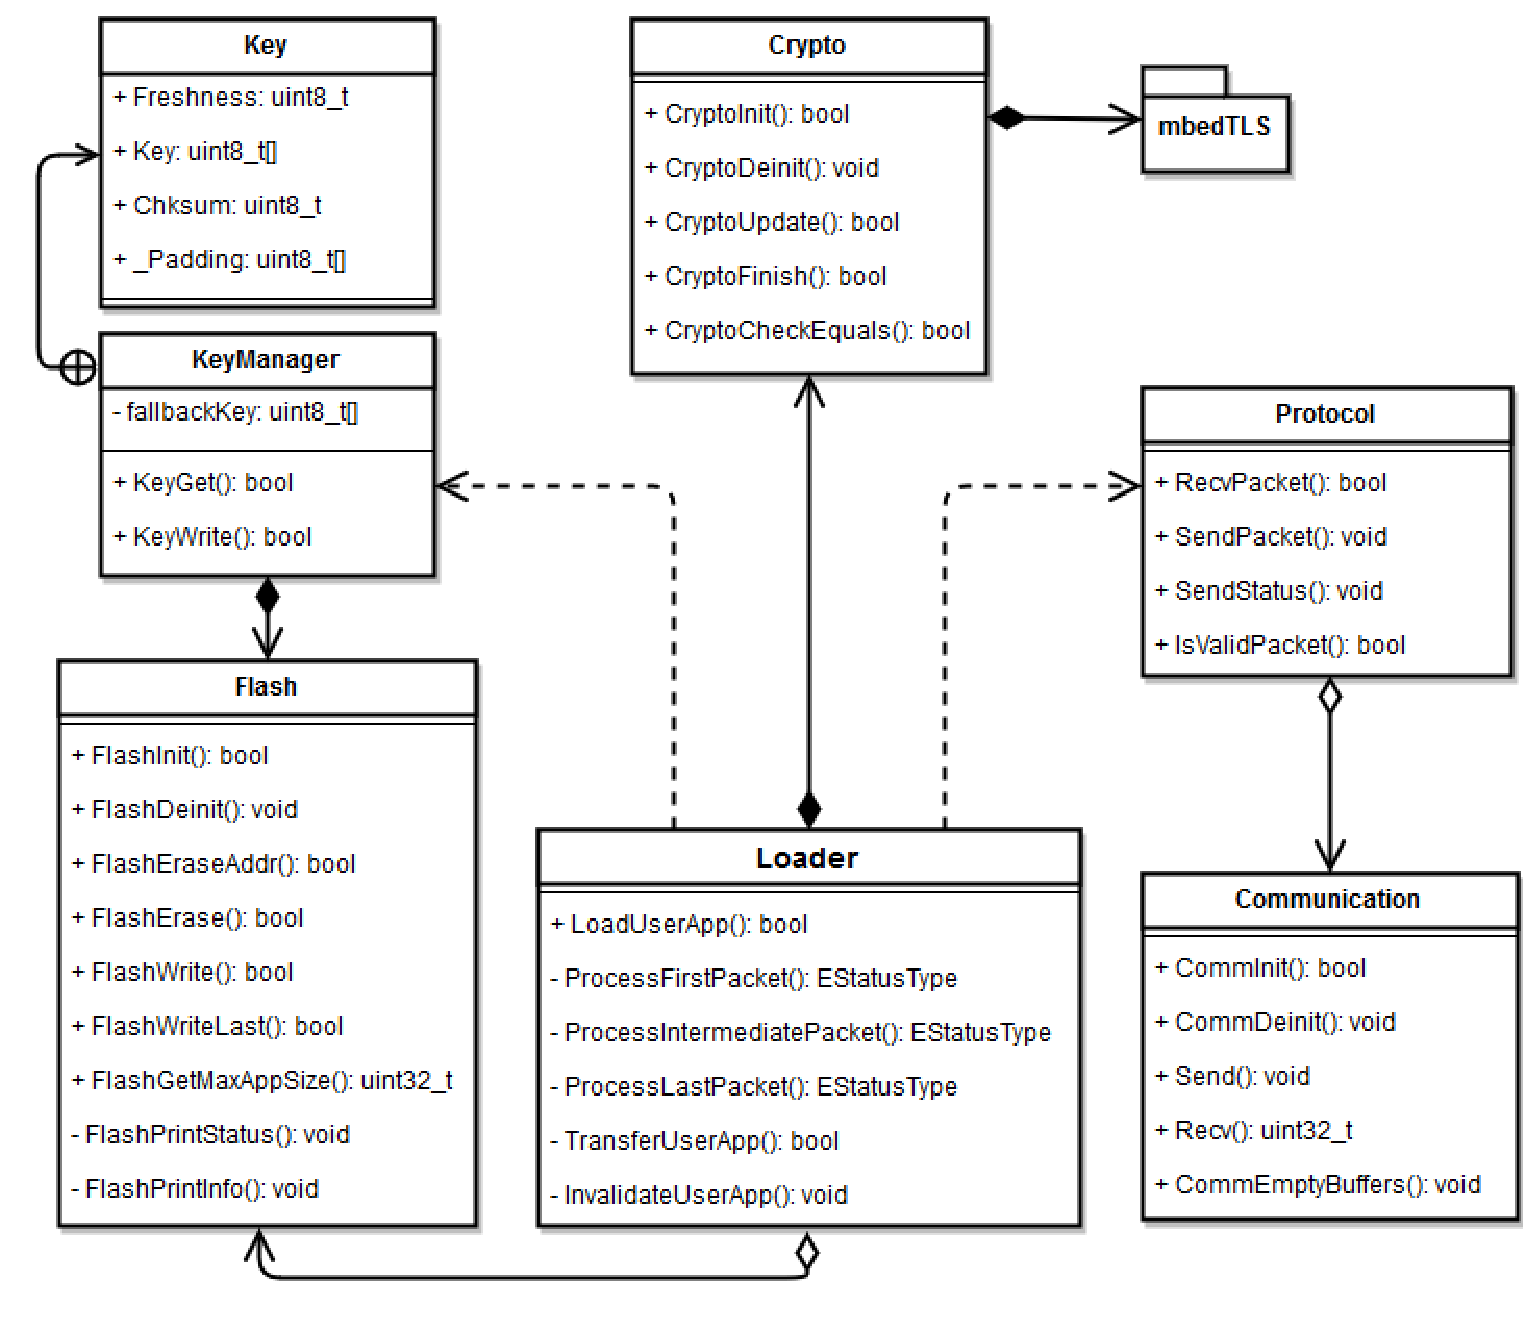
\includegraphics[width=1\textwidth]{arhitectura}
    \caption{Arhitectura modulelor importante ale bootloader-ului}
    \label{arhitectura}
\end{figure}

În această figură distingem modulele:
\begin{itemize}
\item \textbf{Flash}: Folosit la gestionarea scrierii, citirii și ștergerii memoriei flash a microcontroller-ului.
\item \textbf{Crypto}: Are rolul de a gestiona biblioteca de criptare, deci servește ca un strat în plus de abstractizare.
\item \textbf{Communication}: Implementează canalul de comunicație. Acest modul este responsabil cu deschiderea portului serial, trimiterea și primirea de date pe acesta și, bine-înțeles cu închiderea lui.
\item \textbf{Protocol}: Împachetează și formatează datele în pachete pentru a facilita comunicarea așa cum a fost ea descrisă în secțiunea aferentă protocolului de date.
\item \textbf{KeyManager}: Responsabil cu scrierea și citirea cheilor de criptare în zona de memorie rezervată lor.
\item \textbf{Loader}: Modulul principal al aplicației, el le aduce împreună pe restul, punându-le în funcțiune.
\end{itemize}

\subsubsection{Modulul Flash}
În modulul \texttt{Flash} al bootloader-ului se gestionează, conform numelui, memoria flash a microcontroller-ului. Acest modul are codul în fișierele \texttt{Flash.h} și respectiv \texttt{Flash.c}.

Conform interfeței publice acestui modul el pune la dispoziție următoarele funcții:
\begin{itemize}
\item \texttt{bool FlashInit(const uint32\_t u32StartAddress)}: Se ocupă cu inițializarea acestui modul. Argumentul reprezintă adresa de start de unde dorim să facem scrierile. Orice scriere va avansa un pointer intern, iar scrierile următoare vor avea loc de la noua adresă.
\item \texttt{void FlashDeinit()}: Modulul și pointer-ul de adresă de scriere intern sunt eliberate.
\item \texttt{bool FlashEraseAddr(const uint32\_t u32Addr, const uint32\_t u32Len)}: Șterge o zonă de memorie de o anumită lungime, de la o anumită adresă, oriunde în memoria flash.
\item \texttt{bool FlashErase(const uint32\_t u32Len)}: Șterge o zonă de memorie de o anumită lungime începând de la adresa indicată de pointer-ul intern.
\item \texttt{bool FlashWrite(const uint8\_t *pu8Data, const uint32\_t u32Len)}: Scrie date de o lungime dată începând cu adresa indicată de pointer-ul intern și avansează pointer-ul cu lungimea datelor. Lungimea datelor este necesar să fie un multiplu de \texttt{FLASH\_WRITE\_SIZE} (constantă publică definită în interiorul modulului), limitare impusă din nou de partea hardware a memoriei. 
\item \texttt{bool FlashWriteLast(const uint8\_t *pu8Data, const uint32\_t u32Len)}: Asemănător cu funcția de mai sus, diferența este că aceasta funcție adaugă padding la finalul datelor dacă acestea nu sunt un multiplu de \texttt{FLASH\_WRITE\_SIZE}. Numele provine de la faptul că funcția este proiectată să scrie ultima bucată de date, inițial șirul de date fiind împărțit în bucăți care respectă regula, iar ultima bucată necesitând padding.
\item \texttt{uint32\_t FlashGetMaxAppSize()}: Returnează care este dimensiunea maximă a aplicației utilizator care poate fi scrisă în memorie.
\end{itemize}

\subsubsection{Modulul Crypto}
Modulul \texttt{Crypto} este layer-ul de abstractizare al bibliotecii de criptare mbedTLS, aleasă anterior pentru a cripta și respectiv decripta aplicațiile utilizator.

Interfața publică a acestuia pune la dispoziție următoarele funcții:
\begin{itemize}
\item \texttt{bool CryptoInit(bool bEncrypt, const uint8\_t *pu8Iv, const uint8\_t *pu8Key, const uint8\_t u8KeyLength)}: Determină inițializarea modulului de criptografie în modul de criptare sau decriptare în funcție de primul argument. Inițializarea se face cu vectorul de inițializare primit de la utilitarul Flasher în antetul firmware-ului și cu cheia de criptare citită cu ajutorul modulului \texttt{KeyManager}.
\item \texttt{void CryptoDeinit()}: Oprește și eliberează resursele alocate de modul.
\item \texttt{bool CryptoUpdate(const uint8\_t *pu8Data, const uint32\_t u32Len, uint8\_t *pu8Output)}: Apelul acestei funcții declanșează criptarea sau decriptarea datelor pasate ca parametru. Rezultatul este scris în buffer-ul de output, care trebuie să fie alocat în memorie de codul apelant.
\item \texttt{bool CryptoFinish(const uint8\_t *pu8Data, const uint32\_t u32Len, uint8\_t *pu8Output, uint8\_t *pu8Tag, const uint32\_t u32TagLen)}: Încheie criptarea sau decriptarea datelor, generând ultimul rezultat și tag-ul de autentificare necesar validării autenticității datelor.
\item \texttt{bool CryptoCheckEquals(const uint8\_t *pu8Data1, const uint8\_t *pu8Data2, const uint32\_t u32Len)}: Implementează comparația a două șiruri de date în timp constant, așa cum a fost descris într-o secțiune anterioară.
\end{itemize}

În cadrul acestui modul este interesant de prezentat modul flux al algoritmului AES, lucrul cu acest mod fiind prezentat în listing-ul \ref{aesStream}.

\begin{listing}[h]
\begin{minted}{c}
/* ... */

bRetval = (0 == mbedtls_gcm_update(&_ctx, u32Len,
                                   pu8Data, pu8Output));

if(bRetval)
{
    bRetval = (0 == mbedtls_gcm_finish(&_ctx, pu8Tag, u32TagLen));
    
    /* ... */
}

/* ... */
\end{minted}

\caption{O fracțiune a funcției \texttt{CryptoFinish}}
\label{aesStream}
\end{listing}

Dinn listing-ul \ref{aesStream} se observă cum modulul de criptografie este într-adevăr un strat de abstractizare mai înalt pentru biblioteca din spate. Modul flux al algoritmului de criptare constă doar în pasarea segmentată a datelor funcției de update (\texttt{mbedtls\_gcm\_update}), iar la final generarea tag-ului de autentificare (\texttt{mbedtls\_gcm\_finish}), operații care în modul bloc s-ar fi făcut într-un singur apel al funcției \texttt{mbedtls\_gcm\_crypt\_and\_tag} sau \texttt{mbedtls\_gcm\_auth\_decrypt}, așa cum a fost prezentat la începutul acestei lucrări.

\subsubsection{Modulul Communication}
Acest modul este cel care permite comunicația bootloader-ului pe portul serial, acesta făcând posibilă trimiterea și primirea datelor prin interfața sa publică:
\begin{itemize}
\item \texttt{bool CommInit()}: Inițializează și deschide portul serial de comunicație.
\item \texttt{void CommDeinit()}: Închide portul serial.
\item \texttt{void Send(const uint8\_t *pu8Data, const uint32\_t u32Len)}: Declanșează trimiterea unui șir de date de o anumită lungime. Apelul acestei funcții returnează abia în momentul în care toate datele au fost trimise spre portul de comunicație.
\item \texttt{uint32\_t Recv(uint8\_t *pu8Data, const uint32\_t u32Len, uint32\_t *pu32Timeout)}: Așteaptă primirea de date de pe portul serial, datele urmând a fi scrise în primul argument, un buffer deja alocat de codul apelant. Acest apel va fi întrerupt dacă după un timp de timeout datele de lungimea cerută nu sosesc.
\item \texttt{void CommEmptyBuffers()}: Echivalentul unei reinițializări. Forțează modulul să golească buffer-ele interne folosite la citirea datelor.
\end{itemize}

Un aspect interesant al acestui modul este faptul că primirea datelor se face folosind sistemul de întreruperi al microcontroller-ului. Portul serial fiind capabil să genereze o întrerupere atunci când are loc un eveniment. Codul de tratare al întreruperii este prezentat în listing-ul \ref{uartIRQ}.

\begin{listing}[h]
\begin{minted}{c}
void COMM_IRQHandler()
{
  // check if new data arrived
  if ((kUART_RxDataRegFullFlag | kUART_RxOverrunFlag) &
      UART_GetStatusFlags(COMM_UART))
  {
      uint8_t u8Data = UART_ReadByte(COMM_UART);

      // if the ring buffer is not full, add data to it
      if (!RbIsFull())
      {
          RbWrite(u8Data);
      }
      else
      {
          LOG_ERR("Ring buffer full!");
      }
  }
}

\end{minted}

\caption{Codul rutinei de tratare a întreruperii aferentă portului serial}
\label{uartIRQ}
\end{listing}

Această rutină verifică dacă întreruperea a fost generată din cauza primirii a noi date pe port, iar dacă acest lucru este adevărat, citește octetul sosit și îl pune într-un buffer circular. Buffer-ul circular este necesar pentru a gestiona caracterele primite până la un moment dat și pentru a evita alocarea de memorie pentru fiecare citire. Buffer-ul acesta va fi prezentat într-o secțiune următoare, drept un modul auxiliar al bootloader-ului.

\subsubsection{Modulul Protocol}
Mai sus am arătat pe scurt cum se folosește modulul de comunicație, acesta permițând trimiterea de date și primirea lor pe portul serial. Datele trimise și primite de bootloader vor avea un anumit format, acest format este stabilit de modulul \texttt{Protocol}. În urma împachetării datelor, conform protocolului prezentat într-o secțiune anterioară, se vor folosi funcțiile modulului \texttt{Communication} pentru a trimite pachetul pe portul serial.

Interfața publică a acestui modul este:
\begin{itemize}
\item \texttt{bool RecvPacket(uint8\_t *pu8Data, uint32\_t *pu32Len, EPacketType *peType, uint32\_t u32Timeout)}: Similar cu funcția \texttt{Recv} din modulul de comunicație, această funcție așteaptă să primească un pachet pe linia serială. Din pachet se vor extrage datele utile, împreună cu lungimea lor, cât și tipul pachetului care a sosit. Această funcție poate aștepta și ea un timeout până când pachetul poate fi primit.
\item \texttt{void SendPacket(const uint8\_t *pu8Data, const uint32\_t u32Len, const EPacketType ePacketType)}: Trimite anumite date pe portul serial, împachetându-le într-un anumit tip de pachet.
\item \texttt{void SendStatus(const EStatusType eStatus)}: Trimite un pachet de tip \texttt{STATUS\_PACKET}, cu un anumit status pe portul serial. Această funcție este folosită de bootloader pentru a indica starea transmisiunii până la un punct în timp.
\end{itemize}

Conform semnăturilor funcțiilor acest modul definește și tipurile înfățișate în listing-ul \ref{protocolTypes};
\begin{listing}[h]
\begin{minted}{c}
enum EPacketType_
{
    FIRST_PACKET = 0x00,
    NEXT_PACKET,
    LAST_PACKET,
    STATUS_PACKET,
};
typedef enum EPacketType_ EPacketType;

enum EStatusType_
{
    STATUS_ACK = 0x00,
    STATUS_ERROR,
    STATUS_RETRY,
    STATUS_SUCCESS,
};
typedef enum EStatusType_ EStatusType;

#pragma pack(push, 1)
struct TPacketHeader_
{
    uint16_t m_u16Id;
    uint8_t m_u8Type;
    uint8_t m_u8Length;
};

typedef struct TPacketHeader_ TPacketHeader;
#pragma pack(pop)
\end{minted}

\caption{Tipurile definite de modulul \texttt{Protocol}}
\label{protocolTypes}
\end{listing}

Listing-ul \ref{protocolTypes} poate fi considerat oglinda celor prezentate în secțiunea care descrie pe larg comportamentul protocolului. Se poate vedea în primul rând care sunt tipurile de pachet pe care bootloader-ul le poate trimite sau accepta: \texttt{FIRST\_PACKET}, \texttt{NEXT\_PACKET}, \texttt{LAST\_PACKET}, \texttt{STATUS\_PACKET}, acestea fiind stocate în câmpul \texttt{m\_u8Type} al antetului pachetului.
Avem de asemenea definite și codurile de stare, de la \texttt{STATUS\_ACK}, până la \texttt{STATUS\_SUCCESS}.

Antetul pachetului constă din structura \texttt{TPacketHeader} și arată exact așa cum a fost el prezentat în secțiunea dedicată protocolului. Singurul lucru care nu este descris de această structură este modul cum se așează datele după antet și mai important cum se atașează codul polinomial de 16 biți la finalul datelor din pachet. Prezint bucata de cod care face acest lucru în listing-ul \ref{SendPacket}.

\begin{listing}[h]
\begin{minted}{c}
void SendPacket(const uint8_t *pu8Data, const uint32_t u32Len,
                const EPacketType ePacketType)
{
  uint8_t au8Packet[256];

  TPacketHeader *packetHeader = (TPacketHeader *)au8Packet;
  packetHeader->m_u16Id = PACKET_ID;
  packetHeader->m_u8Type = ePacketType;
  packetHeader->m_u8Length = u32Len;

  memcpy(au8Packet + sizeof(TPacketHeader), pu8Data, u32Len);
  uint16_t u16Crc = Crc16Ccitt(pu8Data, u32Len);
  memcpy(au8Packet + sizeof(TPacketHeader) + u32Len, &u16Crc, 2);

  // size = header + data + crc
  Send(au8Packet, sizeof(TPacketHeader) + u32Len + 2);
}
\end{minted}

\caption{Funcția \texttt{SendPacket} a modulului \texttt{Protocol}}
\label{SendPacket}
\end{listing}

O instanță a structurii de tipul \texttt{TPacketHeader} este populată cu datele necesare, instanța fiind suprapusă unui buffer de memorie \texttt{au8Packet} de ajuns de mare încât să poată memora un întreg pachet. În urma populării antetului, se copiază datele transportate de pachet și apoi se calculează codul polinomial CRC-16 peste datele utile, codul polinomial fiind apoi atașat la finalul pachetului. În cele din urmă, funcția \texttt{Send} a modulului \texttt{Communication} este folosită pentru a trimite întregul pachet pe portul serial.

Datorită modularizării codului, dacă pe viitor se dorește comunicația și în alte medii, de exemplu folosind TCP/IP, tot ce trebuie să facă programatorul este să reimplementeze codul modulului de comunicație, iar dacă interfața rămâne neschimbată, atunci și modulul \texttt{Protocol} poate fi reutilizat.

\subsubsection{Modulul KeyManager}

Modulul \texttt{KeyManager} este important datorită faptului că acesta se ocupă cu citirea cheilor din memoria flash a  microcontroller-ului. Acest modul are următoarea interfață publică:

\begin{itemize}
\item \texttt{bool KeyGet(uint8\_t *pu8Key, uint8\_t *pu8Freshness)}: Citește o cheie de criptare din memorie și o scrie în primul argument pasat funcției, acest argument trebuie să fie deja alocat și destul de încăpător pentru o cheie de criptare (16 octeți).
\item \texttt{bool KeyWrite(const uint8\_t u8Freshness, const uint8\_t *pu8Key, const uint8\_t u8Index)}: Implementează codul de scriere al unei chei de criptare, aceasta va fi scrisă la poziția indicată de ultimul argument, cu un indice de prospețime atât cât spune primul parametru.
\end{itemize}

Deși interfața sa publică pune la dispoziție și o funcție de scriere a unei chei de criptare, bootloader-ul nu o folosește. Această funcție a fost scrisă din considerente de reutilizare a codului, acest modul putând fi reutilizat de o aplicație utilizator care face scrierea cheilor.

Cele două funcții, de citire și respectiv scriere, ambele cer un argument numit "freshness". Funcția de citire scrie acest argument, folosind-ul ca argument de ieșire, iar cea de scriere a unei chei, citește acest argument pentru a-l scrie în memoria flash, fără să îl modifice. Freshness-ul, reprezintă prospețimea unei chei de criptare, cu cât el are o valoare mai mare, cu atât bootloader-ul, respectiv funcția \texttt{KeyGet}, consideră că o cheie este mai nouă. Acest parametru a fost introdus pentru a putea face distincția între diferitele chei stocate pe microcontroller.
Planul inițial fiind simplu și considerând o singură cheie de criptare nu ar fi necesitat un asemenea indicator. Totuși pentru că am mărit spațiul rezervat unei chei de criptare la un întreg sector (din considerente hardware), am decis să introduc acest indice de prospețime pentru a putea alege o cheie de criptare dintre toate cele existente în zona dedicată lor.

În mod artificial am limitat numărul de chei de criptare la două, deoarece avem nevoie doar de o singură cheie de criptare și eventual de una de rezervă, nefiind nevoie de mai multe chei pentru că acestea se pot schimba. Bootloader-ul va prefera tot timpul o cheie de criptare cu un freshness mai mare, aceasta fiind considerată mai nouă.

O aplicație utilizator care schimbă aceste chei poate folosi freshness-ul în avantajul său. Dacă pe microcontroller există două chei, una pe prima poziție (\texttt{u8Index = 0}) cu freshness-ul 1 și una pe poziția a doua cu freshness-ul 0, inițial bootloader-ul va prefera cheia de pe poziția 0, având un indicator de prospețime mai mare. Când o aplicație dorește să schimbe a doua cheie și să îi seteze un freshness de 2, ar trebui să suprascrie datele din zona de memorie rezervată cheilor. În caz că scrierea noii chei nu se încheie cu succes, se poate întrerupe alimentarea microcontroller-ului de exemplu, indicatorul de freshness al primei chei este neschimbat, așadar, chiar dacă scrierea noii chei a eșuat, bootloader-ul poate funcționa în continuare folosind tot prima cheie.

Structura unei chei care este stocată în memorie arată ca în listing-ul \ref{keyStruct}.

\begin{listing}[h]
\begin{minted}{c}
#pragma pack(push, 1)
struct TKey_
{
    uint8_t m_u8Freshness;
    uint8_t m_au8Key[KEY_LEN];
    uint8_t m_u8Chksum;
    uint8_t _au8Padding[/* ... */];
};
#pragma pack(pop)
\end{minted}

\caption{Structura din memorie a unei chei de criptare}
\label{keyStruct}
\end{listing}

În plus față de ceea ce am descris deja, listing-ul acesta ne mai arată și faptul că am folosit și aici un cod polinomial de detecție a erorilor, acesta fiind util în cazul în care memoria flash devine coruptă. Bootloader-ul va alege tot timpul cheia cea mai proaspătă (un indicator de prospețime mare) și care are și CRC-ul valid. Ultimul membru al structurii are rolul de a adăuga atât padding cât este necesar pentru ca toată structura să ajungă la mărimea minimă care poate fi ștearsă din memoria flash. Aplicația utilizator folosind această funcționalitate pentru a schimba cheile. Fiind vorba de o memorie flash, cheia trebuie întâi ștearsă și abia apoi scrisă valoarea noii chei.

\subsubsection{Modulul Loader}

Acesta este modulul principal al bootloader-ului, după cum se vede și în diagrama UML el folosește funcționalitatea tuturor celorlalte module, fie în mod direct, cum este cazul modulelor \texttt{KeyManager}, \texttt{Protocol}, \texttt{Crypto} și \texttt{Flash}, fie indirect cum este cazul modulului \texttt{Communication} sau a bibliotecii mbedTLS.

Unica funcție publică a acestui modul este \texttt{bool LoadUserApp()}, ea este responsabilă pentru a încărca aplicația utilizator. Dacă la transfer apare o eroare sau se constată că aplicația nu este autentică, tot această funcție va determina invalidarea zonei de memorie a aplicației, pentru a evita executarea unei aplicații malițioase sau invalide data viitoare când microcontroller-ul pornește. Așadar doar în acest scurt scenariu observăm că modulul \texttt{Loader} folosește funcția \texttt{FlashEraseAddr} a modulului \texttt{Flash} pentru a invalida o porțiune a memoriei flash și funcția \texttt{CryptoCheckEquals} a modulului \texttt{Crypto} pentru a valida tag-ul de autentificare al aplicației tocmai transferate.

Funcționarea acestui modul poate fi privită ca un automat cu stări finite, așa cum este ilustrat în figura \ref{loaderStates}.

\begin{figure}[h]
    \centering
    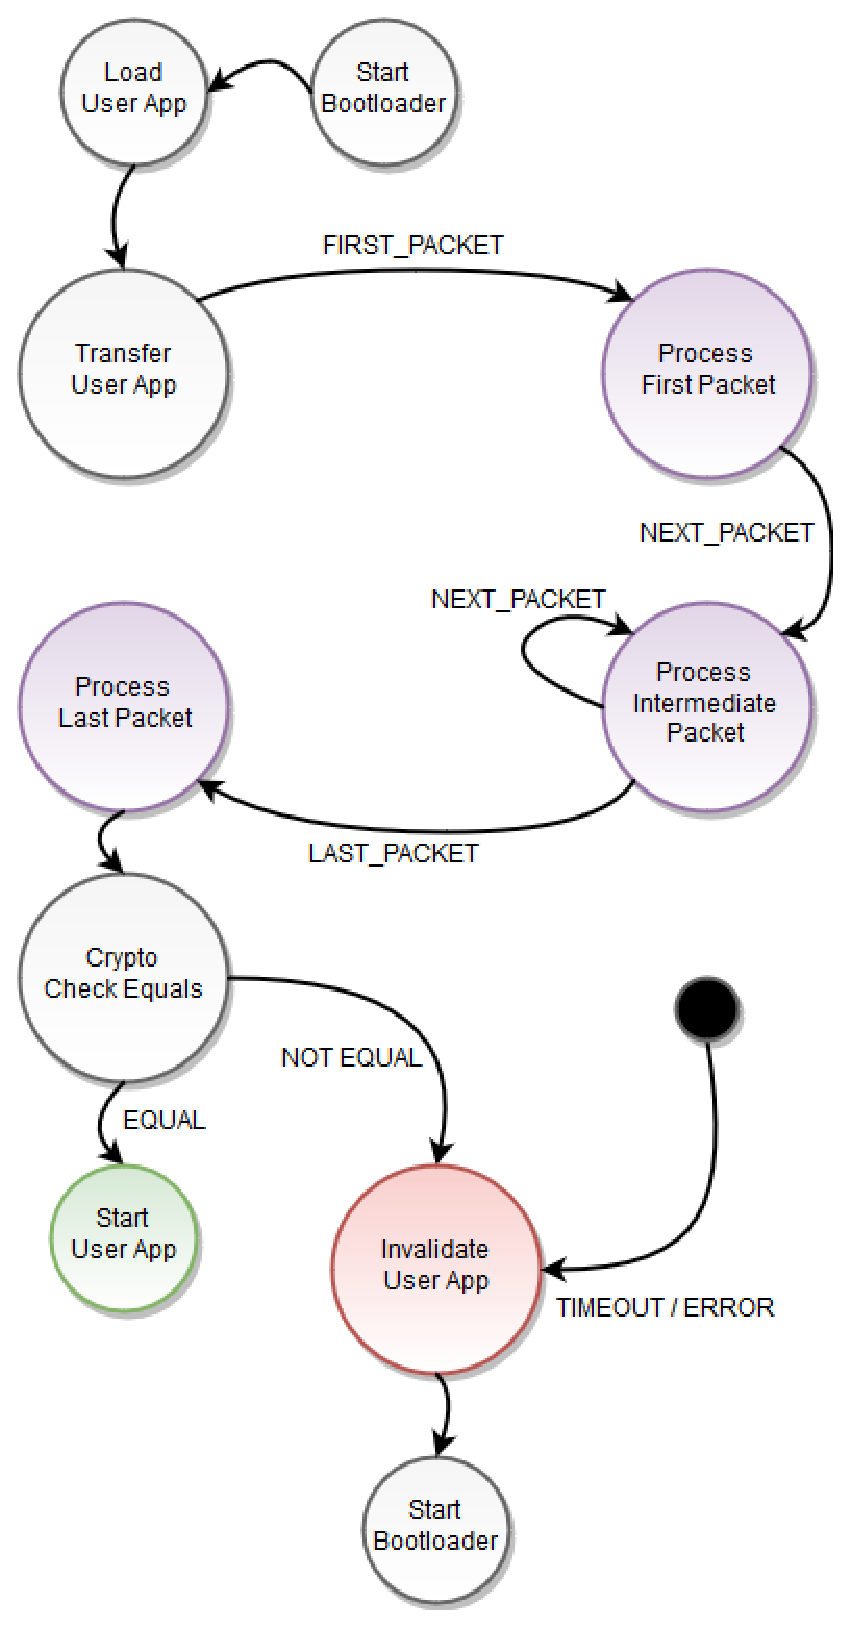
\includegraphics[width=0.7\textwidth]{loader_states}
    \caption{Fluxul de date în modulul \texttt{Loader}}
    \label{loaderStates}
\end{figure}

Datorită faptului ca întreg fluxul de date este determinat de transmisia pe portul serial, această figură este extrem de asemănătoare cu ceea ce am prezentat în secțiunea dedicată protocolului de comunicație. Tranzițiile între stările automatului făcându-se în mare parte datorită sosirii anumitor tipuri de pachete. Aceste stări au fost reprezentate cu culoarea mov. Pe când stările gri reprezintă stări necondiționate de o tranziție, ele putând fi la fel de bine încorporate în starea anterioară sau următoare a grafului, dar au fost păstrate separate pentru a înfățișa cât mai bine comportamentul bootloader-ului.

În cazul în care codul va ajunge în starea de "Start User App", bootloader-ul a primit cu succes o aplicație validă, și va continua cu execuția aplicației.
În caz contrar, când apare o eroare sau aplicația este invalidă, bootloader-ul va încerca să reia procesul de la început.
Toate stările prezentate pe acest graf reprezintă nume de funcții din modulele \texttt{Loader} și \texttt{Crypto}, dar și funcții din fișierul \texttt{main.c}: \texttt{void StartBootloader()} și \texttt{void StartUserApp()}.
Starea "Start User App" fiind chiar starea pe care ne-o dorim.

Cele două funcții din \texttt{main.c} reprezintă punctele principale de intrare la pornirea microcontroller-ului, dacă pe microcontroller există deja o aplicație validă și utilizatorul nu apasă butonul hardware, aplicația va fi pornită prin apelarea funcției \texttt{StartUserApp}, dacă în schimb utilizatorul apasă pe butonul dispozitivului sau nu există o aplicație validă la pornirea sistemului embedded, bootloader-ul va fi pornit prin apelul funcției \texttt{StartBootloader}, moment în care acesta va iniția modulele de criptografie, cel de lucru cu memoria (\texttt{Flash}), modulul de comunicație și va aștepta transmisia unei aplicații pe portul serial.

Rutina \texttt{StartUserApp} nu face decât să apeleze punctul de intrare al aplicației utilizator. Adresa rutinei de intrare este citită din memorie, de la un offset fix față de începutul aplicației, conform memory map-ului. În urma setării pointer-ului se apelează funcția de la adresa respectivă. Această secvență de cod este prezentată în listing-ul \ref{startUserApp}.

\begin{listing}[h]
\begin{minted}{c}
uint32_t u32UserAppStartRoutineAddr = 
  *((uint32_t *)(USER_APP_START_ADDR + PC_OFFSET));
((void(*)())u32UserAppStartRoutineAddr)();
\end{minted}

\caption{Codul de pornire al aplicației utilizator}
\label{startUserApp}
\end{listing}

Se observă din acest listing faptul că adresa rutinei principale a aplicației se află la \texttt{PC\_OFFSET}, în acest caz, la 4 octeți distanță față de începutul zonei de memorie a aplicației. Această adresă este citită prin convertirea la un pointer, pointer care apoi este dereferențiat ca să ne dea adresa propriu-zisă a funcției de start. În urma aflării adresei funcției de start, apelăm această funcție ca și cum am apela o funcție pasată prin pointer, cele două cazuri fiind echivalente.

\subsection{Modulele auxiliare}

Ca toate lucrurile prezentate mai sus să fie posibile s-au folosit și câteva module auxiliare, acestea nu contribuie efectiv la funcționalitatea de încărcare a aplicației, dar fără ele încărcarea nu ar fi totuși posibilă.

Prezentăm în figura \ref{arhitectura-aux} diagrama UML a acestor module.

\begin{figure}[h]
    \centering
    \includegraphics[width=0.9\textwidth]{arhitectura-aux}
    \caption{Arhitectura modulelor auxiliare ale bootloader-ului}
    \label{arhitectura-aux}
\end{figure}

Din diagramă distingem aceste module auxiliare:
\begin{itemize}
\item \textbf{Hardware}: Modulul responsabil cu gestiunea butonului de pornire al bootloader-ului. Mecanismul pe care acest modul îl folosește este unul simplu: pe un pin al microcontroller-ului se pune semnalul "1" logic, iar un alt pin este setat ca input. În momentul în care cele două sunt legate împreună (prin apăsarea unui buton sau setarea unui jumper) pin-ul de input va citi semnalul "1" logic. Deoarece bootloader-ul este interesat doar de starea pinului la pornire, este de ajuns un simplu if, deoarece starea înaltă a semnalului este păstrată în mod natural de utilizator prin apăsarea continuă a butonului.
\item \textbf{Retarget}: Fiind vorba de un mediu embedded, acest modul redirecționează ieșirea funcției \texttt{printf} pe un port serial special rezervat pentru depanarea programelor care rulează pe microcontroller.
\item \textbf{Crc}: Aici sunt implementate funcțiile care calculează codurile polinomiale așa cum au fost descrise ele în partea de început a acestei lucrări, în cadrul secțiunii cu noțiuni teoretice.
\item \textbf{Timer}: Acest modul vine în ajutorul modulului de comunicație, facilitând măsurarea timpului și implementarea mecanismului de timeout.
\item \textbf{RingBuffer}: Buffer-ul pe care modulul de comunicație îl populează atunci când primește date pe portul serial este implementat de acest modul. Este vorba de un buffer circular, de mărime fixă care evită alocarea de memorie pentru pachetele care vin din exterior.
\end{itemize}

Deoarece restul modulelor au o implementare trivială sau au fost deja prezentate aspectele importante legate de funcționarea lor, așa cum este cazul CRC-ului, voi prezenta în cele ce urmează trei dintre modulele auxiliare.

\subsubsection{Modulul Retarget}
În general, în lumea embedded, prin retargetting se înțelege redirectarea apelurilor \texttt{printf} sau \texttt{scanf} spre altceva decât ecran și tastatură. De exemplu \texttt{printf} poate scrie date pe un port serial, iar \texttt{scanf} poate citi date de pe acest port. Retarget-ul este necesar datorită limitării hardware pe care o impune dispozitivul embedded, acesta neavând un ecran și o tastatură încorporate și în general fiind necesar să ruleze fără asemenea periferice atașate.

În cadrul bootloader-ului modulul \texttt{Retarget} este modulul care se ocupă doar cu redirectarea funcției \texttt{printf}. Acest lucru se face prin redefinirea a două funcții din biblioteca standard a C-ului \cite{retarget}: \texttt{int \_write(int fd, const void *buf, size\_t count)} și \texttt{int fputc(int ch, FILE *f)}. Noile implementări sunt vizibile în listing-ul \ref{retargetCode}.

\begin{listing}[h]
\begin{minted}{c}
int fputc(int ch, FILE *f)
{
    UartSendChar(ch);
    return ch;
}

int __attribute__((used)) _write(int fd,
    const void *buf, size_t count)
{
    for(size_t i=0; i< count; ++i)
    {
        UartSendChar(((char *)buf)[i]);
    }

    return count;
}
\end{minted}

\caption{Codul de retarget al bootloader-ului}
\label{retargetCode}
\end{listing}

Cele două funcții își păstrează comportamentul conform interfeței lor, \texttt{fputc} trimite un singur caracter spre portul serial, pe când \texttt{\_write} scrie un întreg buffer. Totuși ambele funcții au în comun apelul la funcția \texttt{UartSendChar}. Aceasta fiind de fapt cea care face trimiterea pe serial a unui octet de date. Implementarea ei poate fi găsită în fișierul \texttt{Retarget.c} la un loc cu cele două funcții descrise anterior.

\subsubsection{Modulul Timer}
Modulul \texttt{Timer} este cel care implementează funcționalitatea de timeout folosită în cadrul comunicației.
Acesta, prin interfața sa publică, permite pornirea unui cronometru și verificarea acestuia:

\begin{itemize}
\item \texttt{void TimerInit()}: Pornește modulul de cronometrare, dar nu pornește și cronometrul.
\item \texttt{void TimerDeinit()}: Oprește modulul de cronometrare și eliberează resursele acestuia.
\item \texttt{void TimerStart(const uint32\_t u32Timeout)}: Pornește cronometrul, acesta cronometrând până ajunge la numărul de milisecunde specificate ca parametru după care oprindu-se singur.
\item \texttt{uint32\_t TimerStop()}: Oprește cronometrul dacă acesta nu s-a oprit singur.
\item \texttt{bool TimerIsExpired()}: Verifică dacă cronometrul a fost oprit sau a expirat.
\end{itemize}

Deoarece cronometrul trebuie să ruleze și dacă procesorul este ocupat cu executarea de cod util, acest modul folosește și el, ca și modulul de comunicație, întreruperile. În funcția \texttt{TimerStart} întreruperea este pornită și timeout-ul este setat, iar în \texttt{TimerStop} întreruperea este dezactivată și timpul care a mai rămas până când întreruperea ar fi fost declanșată, este returnat. Codul rutinei de tratare a întreruperii este cât se poate de simplu, el poate fi văzut în listing-ul \ref{timerIrq}.

\begin{listing}[h]
\begin{minted}{c}
void PIT0_IRQHandler()
{
    _bTimeout = true;
    TimerStop();
}
\end{minted}

\caption{Rutina de tratare a întreruperii de cronometru}
\label{timerIrq}
\end{listing}

Această rutină face doar să marcheze faptul că perioada de cronometrare setată la apelul \texttt{TimerStart} a fost atinsă și apoi să oprească cronometrul. \texttt{PIT} vine de la "Periodic Interrupt Timer", componenta hardware pe care se bazează acest modul și care oferă de fapt funcționalitatea și oscilatorul pentru măsurarea timpului \cite{kv5x}.

\subsubsection{Modulul RingBuffer}

Pentru a evita alocarea memoriei dinamice (pe heap), modulul \texttt{RingBuffer} vine cu o implementare de buffer circular pe care modulul \texttt{Communication} o folosește pentru a stoca datele care vin de pe portul serial.

Interfața publică a acestui modul este:
\begin{itemize}
\item \texttt{bool RbInit(volatile uint8\_t *pu8RingBuffer, const uint32\_t u32RingBufferSize)}: Inițializează un buffer circular de o anumită lungime în zona de memorie specificată prin cei doi parametrii.
\item \texttt{void RbDeinit()}: Resetează buffer-ul circular.
\item \texttt{uint32\_t RbRead(uint8\_t *pu8Data, const uint32\_t u32Len)}: Citește din buffer-ul circular un șir de date de lungimea indicată de al doilea parametru și îl scrie în buffer-ul indicat de primul argument.
\item \texttt{void RbWrite(const uint8\_t u8Data)}: Adaugă date în buffer, cu riscul de a suprascrie date vechi dacă lungimea celor noi ar trece de finalul curent al bootloader-ului
\item \texttt{bool RbIsFull()}: Verifică daca buffer-ul circular este plin.
\item \texttt{uint32\_t RbCount()}: Returnează lungimea datelor care sunt stocate în mod curent în buffer.
\item \texttt{void RbEmpty()}: Golește buffer-ul circular.
\end{itemize}

Un buffer circular este foarte util în mediul embedded deoarece nu necesită foarte multe resurse pentru a fi implementat. O zonă de memorie care să țină datele și doi pointer-i, unul la capătul de scriere și unul la capătul de citire al buffer-ului ajung pentru a avea o implementare eficientă. De asemenea această structură de date este preferată deoarece golirea sa se face în timp constant (implică doar resetarea a celor doi pointeri la începutul zonei de memorie) și deci modulul de comunicație poate să golească rapid buffer-ul între două trimiteri sau primiri de pachete.

Nu în ultimul rând, în afară de modulele cu o structură și un rol bine definite, bootloader-ul mai este format din două fișiere, \texttt{Config.h} și \texttt{Log.h}. Cele două fișiere sunt incluse la discreție de modulele bootloader-ului pentru a avea acces la adresele de start ale zonelor de memorie, definite drept constante în fișierul \texttt{Config.h}. De asemenea fișierul \texttt{Log.h} este folosit ca un strat subțire de abstractizare peste funcțiile de afișare (care la rândul lor au fost suprascrise de modulul \texttt{Retarget}) oferind informații în plus, cum ar fi linia și fișierul de unde este apelată funcția curentă care face output. Aceste informații au fost vitale în depanarea bootloader-ului și în timpul dezvoltării sale acesta fiind singurul mod de a ști care a fost ultimul loc vizitat de microprocesor înainte să apară o problemă.

\section{Structura utilitarelor Flasher și Bundler}
În cele ce urmează voi prezenta succint structura utilitarelor dezvoltate pentru PC, cele care vin în completarea bootloader-ului. Datorită modularizării codului de la bootloader, aceste două utilitare vor refolosi o parte din codul scris pentru bootloader. Utilitarele, datorită faptului că rulează pe arhitecturi x86 și x64 și nu sunt constrânse de spațiu, au fost scrise în limbajul C++, limbaj ales datorită ușurinței cu care putem să apelăm cod C, pentru a putea refolosi codul bootloader-ului.

Bundler-ul va trebui să refolosească codul din modulul \texttt{Crypto} deoarece el se ocupă cu crearea fișierului firmware. Crearea acestui fișier presupune criptarea aplicației utilizator. Bundler-ul nu face altceva decât să citească fișierul \texttt{.bin}, să genereze un vector de inițializare pentru algoritmul de criptare și după scrierea antetului în fișierul \texttt{.fw}, să cripteze și să scrie aplicația utilizator.

În listing-ul \ref{genIV} se poate vedea codul de generare al unui vector de inițializare.

\begin{listing}[h]
\begin{minted}{c}
void CBundler::GenerateIV(uint8_t *pu8Iv)
{
  time_t currentTime = time(NULL);
  memcpy(pu8Iv, (void *)&currentTime, sizeof(currentTime));

  srand(currentTime);
  for(int i=sizeof(currentTime); i < CRYPTO_IV_LEN; ++i)
  {
      pu8Iv[i] = rand() % 256;
  }
}
\end{minted}

\caption{Generarea vectorului de inițializare pentru algoritmul AES}
\label{genIV}
\end{listing}

Se poate vedea că generez acest vector folosind numere pseudo-random și timpul curent, deoarece specificația AES recomandă ca acest vector să fie de fiecare dată diferit. Folosind timpul curent acest lucru este deja asigurat.

Deoarece algoritmul AES generează tag-ul de autentificare doar la finalul procesului de criptare, iar antetul fișierului \texttt{.fw} trebuie scris la început, suntem nevoiți să scriem antetul, rezervând spațiu pentru tag-ul de autentificare, iar la finalul procesului să revenim, folosind funcția \texttt{fseek} din biblioteca standard de C și să completăm tag-ul de autentificare în antetul fișierului firmware. Codul descris aici se poate vedea în listing-ul \ref{writeHeader} și \ref{updateHeader}, pentru scrierea și respectiv completarea antetului.

\begin{listing}[h]
\begin{minted}{c}
TFirmwareHeader fwHeader;
memset(&fwHeader, 0xFF, sizeof(fwHeader));

fwHeader.m_u32ApplicationSize = u32ApplicationSize;
memcpy(fwHeader.m_au8Iv, pu8Iv, CRYPTO_IV_LEN);

bRetval = Write((uint8_t *) &fwHeader, sizeof(fwHeader));
\end{minted}

\caption{Scrierea antetului fișierului firmware}
\label{writeHeader}
\end{listing}

\begin{listing}[h]
\begin{minted}{c}
if(fseek(m_pFile, CRYPTO_IV_LEN, SEEK_SET) == 0)
{
    bRetval = Write(pu8Tag, CRYPTO_TAG_LEN);
}
\end{minted}

\caption{Actualizarea tag-ului de autentificare în antetul fișierului firmware}
\label{updateHeader}
\end{listing}

Constanta \texttt{CRYPTO\_IV\_LEN} provine din modulul de criptografie, prezentat anterior, ea reprezintă lungimea vectorului de inițializare. Funcția \texttt{Write} se ocupă cu scrierea în fișierul firmware a datelor pasate ca parametru.

În ceea ce privește structura utilitarului Flasher acesta folosește în principal modulul \texttt{Protocol} al bootloader-ului pentru a crea și interpreta pachetele, care urmează a fi trimise sau primite de pe portul serial. Acest modul este dependent de modulul de comunicare. Lucru care ar putea reprezenta o problemă datorită faptului că Flasher-ul este o aplicație care rulează pe sisteme x86, cu sisteme de operare Windows, modulul \texttt{Communication} nu se poate folosi așa cum este el implementat pentru bootloader. El fiind scris cu mecanisme specifice hardware-ului embedded. În schimb, datorită faptului că am definit clar interfața modulelor, putem să păstram semnăturile funcțiilor și să schimbăm doar implementarea modulului. Ceea ce va duce la păstrarea neschimbată a modulului \texttt{Protocol}.
Flasher-ul folosește de asemenea modulul \texttt{Crc} al bootloader-ului pentru a calcula codul polinomial atașat la finalul oricărui pachet.

\section{Concluzii și dezvoltări ulterioare}

Așadar în cele prezentate anterior am plecat de la ideea de a reduce costurile de dezvoltare a aplicațiilor embedded și de a mări flexibilitatea modului în care aceste aplicații sunt încărcate pe dispozitivele utilizatorilor și am ajuns la o colecție de trei aplicații, bootloader-ul, Flasher-ul și Bundler-ul. Prima fiind destinată dispozitivului embedded, iar cele două din urmă arhitecturilor x86 sau x64.

Bootloaderul este o aplicație încărcată de către dezvoltator pe microcontroller și care nu poate fi înlocuită ușor de către utilizatorii acestuia.
Rolul bootloader-ului este de a încărca la rândul său o altă aplicație pe microcontroller. Aplicația care face de fapt procesarea utilă pentru care a fost proiectat sistemul embedded.
În urma procesului de bootloading ambele aplicații, atât bootloader-ul cât și aplicația utilizator, vor coexista în
memoria flash a microcontroller-ului, conform unui memory map.

Securitatea acestui bootloader este asigurată de algoritmul de criptare cu cheie simetrică AES (Rijndael), algoritm implementat în biblioteca mbedTLS.

Sunt de părere că scopurile propuse au fost atinse prin codul modular și consistent scris în cadrul aplicațiilor dezvoltate în această lucrare. Se poate observa în secțiunea anterioară a lucrării că tot codul respectă notația ungurească\footnote{hungarian notation} pentru denumirea variabilelor și că formatarea codului este consistentă. De asemenea am încercat să documentez toate funcțiile din interfețele modulelor pentru a facilita reutilizarea acestora, lucru care s-a și întâmplat în momentul în care am scris utilitarele Flasher și Bundler.

Totuși, deși bootloader-ul își face treaba pe care a fost proiectat să o facă, există o serie de îmbunătățiri pe care le putem implementa în cadrul dezvoltărilor ulterioare.

O primă astfel astfel de îmbunătățire este inspirată de bootloader-ele pentru sisteme desktop (de exemplu GRUB), aceasta ar consta în alegerea unei aplicații dintre câteva existente în memoria microcontroller-ului. În prezent bootloader-ul poate doar să încarce o singură aplicație în memoria flash. Totuși acestă funcționalitate nu are o implementare evidentă, deoarece utilizatorul va trebui să aleagă o aplicație care să ruleze când microcontroller-ul este pornit, iar perifericele de intrare sunt limitate la sistemele embedded sau inexistente în anumite cazuri.

Deoarece și perifericele de ieșire sunt limitate la anumite sisteme embedded, bootloader-ul ar trebui să își semnalizeze stările prin aprinderea anumitor LED-uri de stare. În cel simplu caz ar trebui să indice doar faptul că rulează și că așteaptă trimiterea unei aplicații pe portul serial.

O altă îmbunătățire, ceva mai importantă, ar fi găsirea unei modalități de a modifica în mod automat o aplicație utilizator să ruleze de la o anumită adresă în memorie. Îmbunătățirea aceasta ar duce la simplificarea procesului de dezvoltare a aplicațiilor pentru bootloader, scriptul de linker nefiind necesar în acest caz.

În ceea ce privește protocolul de comunicație între bootloader și Flasher, acesta ar putea fi modificat să includă și mesaje de eroare în pachetele de tip \texttt{STATUS\_ERROR}. În mod curent cauza erorilor fiind necunoscută.

În ceea ce privește cele două utilitare, consider că Bundler-ul poate primi o funcționalitate nouă de gestiune a cheilor de criptare, pentru a ști ce cheie de criptare este destinată cărui client. În cazul de față dezvoltatorul trebuie să facă gestiunea lor manual, neexistând un sistem care să îi vină în ajutor. De asemenea faptul că cele două utilitare sunt aplicații în linia de comandă, ar putea fi un impediment pentru utilizatorii mai neexperimentați, așadar o altă îmbunătățire de bun augur ar fi adăugarea unei interfețe grafice celor două utilitare. Fiind scrise in C++, interfața se poate adăuga relativ ușor folosind un set de biblioteci precum Qt\footnote{https://www.qt.io/developers/}.

Acestea fiind zise, bootloader-ul, împreună cu Bundler-ul și Flasher-ul pot fi folosite de către un dezvoltator pentru a facilita trimiterea de versiuni noi ale unei aplicații spre client. Fără a fi necesar ca utilizatorul să dispună de hardware special pentru încărcarea acestor noi aplicații pe microcontroller.

%TODO: mesaje mai bune din bundler/flasher
%TODO: modulele, cum ar fi rb-ul, sunt "singleton"

\newpage
\bibliographystyle{plain}
\bibliography{bibliografie}

\end{document}
